\documentclass[]{book}
\usepackage{lmodern}
\usepackage{amssymb,amsmath}
\usepackage{ifxetex,ifluatex}
\usepackage{fixltx2e} % provides \textsubscript
\ifnum 0\ifxetex 1\fi\ifluatex 1\fi=0 % if pdftex
  \usepackage[T1]{fontenc}
  \usepackage[utf8]{inputenc}
\else % if luatex or xelatex
  \ifxetex
    \usepackage{mathspec}
  \else
    \usepackage{fontspec}
  \fi
  \defaultfontfeatures{Ligatures=TeX,Scale=MatchLowercase}
\fi
% use upquote if available, for straight quotes in verbatim environments
\IfFileExists{upquote.sty}{\usepackage{upquote}}{}
% use microtype if available
\IfFileExists{microtype.sty}{%
\usepackage[]{microtype}
\UseMicrotypeSet[protrusion]{basicmath} % disable protrusion for tt fonts
}{}
\PassOptionsToPackage{hyphens}{url} % url is loaded by hyperref
\usepackage[unicode=true]{hyperref}
\hypersetup{
            pdftitle={Lab Manual},
            pdfauthor={Jade Benjamin-Chung, Kunal Mishra, Stephanie Djajadi, Nolan Pokpongkiat, Anna Nguyen},
            pdfborder={0 0 0},
            breaklinks=true}
\urlstyle{same}  % don't use monospace font for urls
\usepackage{natbib}
\bibliographystyle{apalike}
\usepackage{color}
\usepackage{fancyvrb}
\newcommand{\VerbBar}{|}
\newcommand{\VERB}{\Verb[commandchars=\\\{\}]}
\DefineVerbatimEnvironment{Highlighting}{Verbatim}{commandchars=\\\{\}}
% Add ',fontsize=\small' for more characters per line
\usepackage{framed}
\definecolor{shadecolor}{RGB}{248,248,248}
\newenvironment{Shaded}{\begin{snugshade}}{\end{snugshade}}
\newcommand{\KeywordTok}[1]{\textcolor[rgb]{0.13,0.29,0.53}{\textbf{#1}}}
\newcommand{\DataTypeTok}[1]{\textcolor[rgb]{0.13,0.29,0.53}{#1}}
\newcommand{\DecValTok}[1]{\textcolor[rgb]{0.00,0.00,0.81}{#1}}
\newcommand{\BaseNTok}[1]{\textcolor[rgb]{0.00,0.00,0.81}{#1}}
\newcommand{\FloatTok}[1]{\textcolor[rgb]{0.00,0.00,0.81}{#1}}
\newcommand{\ConstantTok}[1]{\textcolor[rgb]{0.00,0.00,0.00}{#1}}
\newcommand{\CharTok}[1]{\textcolor[rgb]{0.31,0.60,0.02}{#1}}
\newcommand{\SpecialCharTok}[1]{\textcolor[rgb]{0.00,0.00,0.00}{#1}}
\newcommand{\StringTok}[1]{\textcolor[rgb]{0.31,0.60,0.02}{#1}}
\newcommand{\VerbatimStringTok}[1]{\textcolor[rgb]{0.31,0.60,0.02}{#1}}
\newcommand{\SpecialStringTok}[1]{\textcolor[rgb]{0.31,0.60,0.02}{#1}}
\newcommand{\ImportTok}[1]{#1}
\newcommand{\CommentTok}[1]{\textcolor[rgb]{0.56,0.35,0.01}{\textit{#1}}}
\newcommand{\DocumentationTok}[1]{\textcolor[rgb]{0.56,0.35,0.01}{\textbf{\textit{#1}}}}
\newcommand{\AnnotationTok}[1]{\textcolor[rgb]{0.56,0.35,0.01}{\textbf{\textit{#1}}}}
\newcommand{\CommentVarTok}[1]{\textcolor[rgb]{0.56,0.35,0.01}{\textbf{\textit{#1}}}}
\newcommand{\OtherTok}[1]{\textcolor[rgb]{0.56,0.35,0.01}{#1}}
\newcommand{\FunctionTok}[1]{\textcolor[rgb]{0.00,0.00,0.00}{#1}}
\newcommand{\VariableTok}[1]{\textcolor[rgb]{0.00,0.00,0.00}{#1}}
\newcommand{\ControlFlowTok}[1]{\textcolor[rgb]{0.13,0.29,0.53}{\textbf{#1}}}
\newcommand{\OperatorTok}[1]{\textcolor[rgb]{0.81,0.36,0.00}{\textbf{#1}}}
\newcommand{\BuiltInTok}[1]{#1}
\newcommand{\ExtensionTok}[1]{#1}
\newcommand{\PreprocessorTok}[1]{\textcolor[rgb]{0.56,0.35,0.01}{\textit{#1}}}
\newcommand{\AttributeTok}[1]{\textcolor[rgb]{0.77,0.63,0.00}{#1}}
\newcommand{\RegionMarkerTok}[1]{#1}
\newcommand{\InformationTok}[1]{\textcolor[rgb]{0.56,0.35,0.01}{\textbf{\textit{#1}}}}
\newcommand{\WarningTok}[1]{\textcolor[rgb]{0.56,0.35,0.01}{\textbf{\textit{#1}}}}
\newcommand{\AlertTok}[1]{\textcolor[rgb]{0.94,0.16,0.16}{#1}}
\newcommand{\ErrorTok}[1]{\textcolor[rgb]{0.64,0.00,0.00}{\textbf{#1}}}
\newcommand{\NormalTok}[1]{#1}
\usepackage{longtable,booktabs}
% Fix footnotes in tables (requires footnote package)
\IfFileExists{footnote.sty}{\usepackage{footnote}\makesavenoteenv{long table}}{}
\usepackage{graphicx,grffile}
\makeatletter
\def\maxwidth{\ifdim\Gin@nat@width>\linewidth\linewidth\else\Gin@nat@width\fi}
\def\maxheight{\ifdim\Gin@nat@height>\textheight\textheight\else\Gin@nat@height\fi}
\makeatother
% Scale images if necessary, so that they will not overflow the page
% margins by default, and it is still possible to overwrite the defaults
% using explicit options in \includegraphics[width, height, ...]{}
\setkeys{Gin}{width=\maxwidth,height=\maxheight,keepaspectratio}
\IfFileExists{parskip.sty}{%
\usepackage{parskip}
}{% else
\setlength{\parindent}{0pt}
\setlength{\parskip}{6pt plus 2pt minus 1pt}
}
\setlength{\emergencystretch}{3em}  % prevent overfull lines
\providecommand{\tightlist}{%
  \setlength{\itemsep}{0pt}\setlength{\parskip}{0pt}}
\setcounter{secnumdepth}{5}
% Redefines (sub)paragraphs to behave more like sections
\ifx\paragraph\undefined\else
\let\oldparagraph\paragraph
\renewcommand{\paragraph}[1]{\oldparagraph{#1}\mbox{}}
\fi
\ifx\subparagraph\undefined\else
\let\oldsubparagraph\subparagraph
\renewcommand{\subparagraph}[1]{\oldsubparagraph{#1}\mbox{}}
\fi

% set default figure placement to htbp
\makeatletter
\def\fps@figure{htbp}
\makeatother

\usepackage{booktabs}
\usepackage{amsthm}
\makeatletter
\def\thm@space@setup{%
  \thm@preskip=8pt plus 2pt minus 4pt
  \thm@postskip=\thm@preskip
}
\makeatother

\title{Lab Manual}
\author{Jade Benjamin-Chung, Kunal Mishra, Stephanie Djajadi, Nolan Pokpongkiat,
Anna Nguyen}
\date{2020-07-13}

\begin{document}
\maketitle

{
\setcounter{tocdepth}{1}
\tableofcontents
}
\chapter{Welcome to our lab!}\label{welcome-to-our-lab}

We are a team of epidemiologists and biostatisticians engaged in global
health research. This lab manual covers our communication strategy and
code of conduct and goes into detail about best practices for data
science. It is a living document that is updated regularly.

This manual was created with input from a large number of team members
and with inspiration from
\href{https://github.com/alylab/labmanual/blob/master/aly-lab-manual.pdf}{other
scientists' lab manuals}. Feel free to draw from this manual (and please
cite it if you do!).

 This work is licensed under a Creative Commons
Attribution-NonCommercial 4.0 International License.

\chapter{Communication and
coordination}\label{communication-and-coordination}

by Jade Benjamin-Chung

These communications guidelines are evolving as we increasingly adopt
Slack, but here some general principles:

\section{Slack}\label{slack}

\begin{itemize}
\tightlist
\item
  Use Slack for scheduling, coding related questions, quick check ins,
  etc. If your Slack message exceeds 200 words, it might be time to use
  email.
\item
  Use channels instead of direct messages unless you need to discuss
  something private.
\item
  Please make an effort to respond to messages that message you (e.g.,
  \texttt{@jade}) as quickly as possible and always within 24 hours.
\item
  If you are unusually busy (e.g., taking MCAT/GRE, taking many exams)
  or on vacation please alert the team in advance so we can expect you
  not to respond at all / as quickly as usual and also
  \href{https://get.slack.help/hc/en-us/articles/201864558-Set-your-Slack-status-and-availability}{set
  your status in Slack} (e.g., it could say ``On vacation'') so we know
  not to expect to see you online.
\item
  Please thread messages in Slack as much as possible.
\end{itemize}

\section{Email}\label{email}

\begin{itemize}
\tightlist
\item
  Use email for longer messages (\textgreater{}200 words) or messages
  that merit preservation.
\item
  Generally, strive to respond within 24 hours hours. As noted above, if
  you are unusually busy or on vacation please alert the team in advance
  so we can expect you not to respond at all / as quickly as usual.
\end{itemize}

\section{Trello}\label{trello}

\begin{itemize}
\tightlist
\item
  Jade will add new cards within our shared Trello board that outline
  your tasks.
\item
  The higher a card is within your list, the higher priority it is.
\item
  Generally, strive to complete the tasks in your card by the date
  listed.
\item
  Use checklists to break down a task into smaller chunks. Sometimes
  Jade will write this for you, but you can also add this yourself.
\item
  Jade will move your card to the ``Completed'' list when it is done.
\end{itemize}

\section{Google Drives}\label{google-drives}

\begin{itemize}
\tightlist
\item
  We mostly use Google Drive to create shared documents with longer
  descriptions of tasks. These documents are linked to in Trello. Jade
  often shares these with the whole team since tasks are overlapping,
  and even if a task is assigned to one person, others may have valuable
  insights.
\item
  Please invite both of Jade's email addresses to any documents you
  create (\href{mailto:jadebc@gmail.com}{\nolinkurl{jadebc@gmail.com}},
  \href{mailto:jadebc@berkeley.edu}{\nolinkurl{jadebc@berkeley.edu}}).
\end{itemize}

\section{Google Calendar / Meetings}\label{google-calendar-meetings}

\begin{itemize}
\tightlist
\item
  We use Google Calendar to set meetings. Please make sure your calendar
  is set up correctly because sometimes you might not receive a specific
  email or Slack message about it -- only a Google Calendar invitation.
\item
  Our meetings start on the hour, not on Berkeley time.
\item
  If you are going to be late, please send a message in our Slack
  channel.
\item
  If you are regularly not able to come on the hour, notify the team and
  we might choose the modify the agenda order or the start time.
\end{itemize}

\chapter{Code of conduct}\label{code-of-conduct}

\section{Lab culture}\label{lab-culture}

It goes without saying that we strive to work in an environment that is
collaborative, supportive, open, and free from discrimination and
harassment, per University policies.

We encourage students / staff of all experience levels to respectfully
share their honest opinions and ideas on any topic. Our group has
thrived upon such respectful honest input from team members over the
years, and this document is a product of years of student and staff
input (and even debate) that has gradually improved our productivity and
overall quality of our work.

\section{Protecting human subjects}\label{protecting-human-subjects}

All lab members must complete
\href{https://cphs.berkeley.edu/quickguideCITItraining.pdf}{CITI Human
Subjects Biomedical Group 1} training and share their certificate with
Jade. She will add team members to relevant Institutional Review Board
protocols prior to their start date to ensure they have permission to
work with identifiable datasets.

One of the most relevant aspects of protecting human subjects in our
work is maintaining confidentiality. For students supporting our data
science efforts, in practice this means:

\begin{itemize}
\tightlist
\item
  If you are using a virtual computer (e.g., Bluevelvet, AWS, GHAP),
  never save the data in that system to your personal computer or any
  other computer without prior permission.
\item
  Do not share data with anyone without permission, including to other
  members of the group, who might not be on the same IRB protocol as you
  (check with Jade first).
\end{itemize}

Remember, data that looks like it does not contain identifiers to you
might still be classified as data that requires special protection by
our IRB or under HIPAA, so always proceed with caution and ask for help
if you have any concerns about how to maintain study participant
confidentiality.

\section{Authorship}\label{authorship}

We adhere to the
\href{http://www.icmje.org/recommendations/browse/roles-and-responsibilities/defining-the-role-of-authors-and-contributors.html}{ICMJE
Definition of authorship} and are happy for team members who meet the
definition of authorship to be included as co-authors on scientific
manuscripts.

\section{Logging hours}\label{logging-hours}

Please use \href{caltime.berkeley.edu}{Caltime} to log your hours. If
you have a non-exempt appointment (this is the default), you need to
punch in when you start working and punch out when you stop working. The
particular hours /days when you work are not important; rather, we
monitor your total hours in a 2-week period. If you have trouble
remembering to punch in/out, please devise a system that works for you
(i.e., set timers / reminders). Please avoid missing punches, and if you
do, please send Jade a Slack message with the time and date you intended
to punch out.

If you have an exempt appointment (this is the case if you also have a
teaching appointment), you do not need to punch in / out. You will be
expected to work, on average, for a certain number of hours per week.

You may log hours for data science team meetings. You may not log hours
for Colford-Hubbard Research Group meetings or commute time, if
applicable.

\chapter{Code repositories}\label{code-repositories}

By Kunal Mishra, Jade Benjamin-Chung, and Stephanie Djajadi

Each study has at least one code repository that typically holds R code,
shell scripts with Unix code, and research outputs (results .RDS files,
tables, figures). Repositories may also include datasets. This chapter
outlines how to organize these files. Adhering to a standard format
makes it easier for us to efficiently collaborate across projects.

\section{Project Structure}\label{project-structure}

We recommend the following directory structure:

\begin{verbatim}
0-run-project.sh
0-config.R
1 - Data-Management/
    0-prep-data.sh
    1-prep-cdph-fluseas.R
    2a-prep-absentee.R
    2b-prep-absentee-weighted.R
    3a-prep-absentee-adj.R
    3b-prep-absentee-adj-weighted.R
2 - Analysis/
    0-run-analysis.sh
    1 - Absentee-Mean/
        1-absentee-mean-primary.R
        2-absentee-mean-negative-control.R
        3-absentee-mean-CDC.R
        4-absentee-mean-peakwk.R
        5-absentee-mean-cdph2.R
        6-absentee-mean-cdph3.R
    2 - Absentee-Positivity-Check/
    3 - Absentee-P1/
    4 - Absentee-P2/
3 - Figures/
    0-run-figures.sh
    ...
4 - Tables/
    0-run-tables.sh
    ...
5 - Results/
    1 - Absentee-Mean/
        1-absentee-mean-primary.RDS
        2-absentee-mean-negative-control.RDS
        3-absentee-mean-CDC.RDS
        4-absentee-mean-peakwk.RDS
        5-absentee-mean-cdph2.RDS
        6-absentee-mean-cdph3.RDS
    ...
.gitignore
.Rproj
\end{verbatim}

For brevity, not every directory is ``expanded'', but we can glean some
important takeaways from what we \emph{do} see.

\section{\texorpdfstring{\texttt{.Rproj}
files}{.Rproj files}}\label{rproj-files}

An ``R Project'' can be created within RStudio by going to
\texttt{File\ \textgreater{}\textgreater{}\ New\ Project}. Depending on
where you are with your research, choose the most appropriate option.
This will save preferences, working directories, and even the results of
running code/data (though I'd recommend starting from scratch each time
you open your project, in general). Then, ensure that whenever you are
working on that specific research project, you open your created project
to enable the full utility of \texttt{.Rproj} files. This also
automatically sets the directory to the top level of the project.

\section{\texorpdfstring{Configuration (`config')
File}{Configuration (config) File}}\label{configuration-config-file}

This is the single most important file for your project. It will be
responsible for a variety of common tasks, declare global variables,
load functions, declare paths, and more. \emph{Every other file in the
project} will begin with \texttt{source("0-config")}, and its role is to
reduce redundancy and create an abstraction layer that allows you to
make changes in one place (\texttt{0-config.R}) rather than 5 different
files. To this end, paths which will be reference in multiple scripts
(i.e.~a \texttt{merged\_data\_path}) can be declared in
\texttt{0-config.R} and simply referred to by its variable name in
scripts. If you ever want to change things, rename them, or even switch
from a downsample to the full data, all you would then to need to do is
modify the path in one place and the change will automatically update
throughout your project. See the example config file for more details.
The paths defined in the \texttt{0-config.R} file assume that users have
opened the \texttt{.Rproj} file, which sets the directory to the top
level of the project.

\section{Order Files and Directories}\label{order-files-and-directories}

This makes the jumble of alphabetized filenames much more coherent and
places similar code and files next to one another. This also helps us
understand how data flows from start to finish and allows us to easily
map a script to its output (i.e.
\texttt{2\ -\ Analysis/1\ -\ Absentee-Mean/1-absentee-mean-primary.R}
=\textgreater{}
\texttt{5\ -\ Results/1\ -\ Absentee-Mean/1-absentee-mean-primary.RDS}).
If you take nothing else away from this guide, this is the single most
helpful suggestion to make your workflow more coherent. Often the
particular order of files will be in flux until an analysis is close to
completion. At that time it is important to review file order and naming
and reproduce everything prior to drafting a manuscript.

\section{Using Bash scripts to ensure
reproducibility}\label{using-bash-scripts-to-ensure-reproducibility}

Bash scripts are useful components of a reproducible workflow. At many
of the directory levels (i.e.~in \texttt{3\ -\ Analysis}), there is a
bash script that runs each of the analysis scripts. This is
exceptionally useful when data ``upstream'' changes -- you simply run
the bash script. See the \protect\hyperlink{unix}{Unix Chapter} for
further details.

After running bash scripts, \texttt{.Rout} log files will be generated
for each script that has been executed. It is important to check these
files. Scripts may appear to have run correctly in the terminal, but
checking the log files is the only way to ensure that everything has run
completely.

\chapter{Coding practices}\label{coding-practices}

by Kunal Mishra and Jade Benjamin-Chung

\section{Organizing scripts}\label{organizing-scripts}

Just as your data ``flows'' through your project, data should flow
naturally through a script. Very generally, you want to:

\begin{enumerate}
\def\labelenumi{\arabic{enumi}.}
\tightlist
\item
  describe the work completed in the script in a comment header
\item
  source your configuration file (\texttt{0-config.R})
\item
  load all your data
\item
  do all your analysis/computation
\item
  save your data.
\end{enumerate}

Each of these sections should be ``chunked together'' using comments.
See
\href{https://github.com/kmishra9/Flu-Absenteeism/blob/master/Master's\%20Thesis\%20-\%20Spatial\%20Epidemiology\%20of\%20Influenza/2a\%20-\%20Statistical-Inputs.R}{this
file} for a good example of how to cleanly organize a file in a way that
follows this ``flow'' and functionally separate pieces of code that are
doing different things.

\section{Documenting your code}\label{documenting-your-code}

\subsection{File headers}\label{file-headers}

Every file in a project should have a header that allows it to be
interpreted on its own. It should include the name of the project and a
short description for what this file (among the many in your project)
does specifically. You may optionally wish to include the inputs and
outputs of the script as well, though the next section makes this
significantly less necessary.

```
\#\#\#\#\#\#\#\#\#\#\#\#\#\#\#\#\#\#\#\#\#\#\#\#\#\#\#\#\#\#\#\#\#\#\#\#\#\#\#\#\#\#\#\#\#\#\#\#\#\#\#\#\#\#\#\#\#\#\#\#\#\#\#\#\#\#\#\#\#\#\#\#\#\#\#\#\#\#\#\#
\# \citet{Organization} - Example Organization \# \citet{Project} -
Example Project \# \citet{Description} - This file is responsible for
{[}\ldots{}{]}
\#\#\#\#\#\#\#\#\#\#\#\#\#\#\#\#\#\#\#\#\#\#\#\#\#\#\#\#\#\#\#\#\#\#\#\#\#\#\#\#\#\#\#\#\#\#\#\#\#\#\#\#\#\#\#\#\#\#\#\#\#\#\#\#\#\#\#\#\#\#\#\#\#\#\#\#\#\#\#\#

```

Consider using RStudio's
\href{https://support.rstudio.com/hc/en-us/articles/200484568-Code-Folding-and-Sections}{code
folding} feature to collapse and expand different sections of your code.
Any comment line with at least four trailing dashes (-), equal signs
(=), or pound signs (\#) automatically creates a code section. For
example:

\begin{verbatim}
# Section 1 ------------------
\end{verbatim}

\textbf{Note}: If your computer isn't able to handle this workflow due
to RAM or requirements, modifying the ordering of your code to
accomodate it won't be ultimately helpful and your code will be fragile,
not to mention less readable and messy. You need to look into
high-performance computing (HPC) resources in this case.

\subsection{Comments in the body of your
script}\label{comments-in-the-body-of-your-script}

Commenting your code is an important part of reproducibility and helps
document your code for the future. When things change or break, you'll
be thankful for comments. There's no need to comment excessively or
unnecessarily, but a comment describing what a large or complex chunk of
code does is always helpful. See
\href{https://github.com/kmishra9/Flu-Absenteeism/blob/master/Master's\%20Thesis\%20-\%20Spatial\%20Epidemiology\%20of\%20Influenza/1b\%20-\%20Map-Management.R}{this
file} for an example of how to comment your code and notice that
comments are always in the form of:

\texttt{\#\ This\ is\ a\ comment\ -\/-\ first\ letter\ is\ capitalized\ and\ spaced\ away\ from\ the\ pound\ sign}

\subsection{Function documentation}\label{function-documentation}

Every function you write must include a header to document its purpose,
inputs, and outputs. For any reproducible workflows, they are essential,
because R is dynamically typed. This means, you can pass a
\texttt{string} into an argument that is meant to be a
\texttt{data.table}, or a \texttt{list} into an argument meant for a
\texttt{tibble}. It is the responsibility of a function's author to
document what each argument is meant to do and its basic type. This is
an example for documenting a function (inspired by
\href{https://www.oracle.com/technetwork/java/javase/documentation/index-137868.html\#format}{JavaDocs}
and R's
\href{https://blog.rstudio.com/2018/10/23/rstudio-1-2-preview-plumber-integration/}{Plumber
API docs}):

\begin{verbatim}
##############################################
##############################################
# Documentation: calc_fluseas_mean
# Usage: calc_fluseas_mean(data, yname)
# Description: Make a dataframe with rows for flu season and site
# and the number of patients with an outcome, the total patients,
# and the percent of patients with the outcome

# Args/Options:
# data: a data frame with variables flu_season, site, studyID, and yname
# yname: a string for the outcome name
# silent: a boolean specifying whether the function shouldn't output anything to the console (DEFAULT: TRUE)

# Returns: the dataframe as described above
# Output: prints the data frame described above if silent is not True

calc_fluseas_mean = function(data, yname, silent = TRUE) {
 ### function code here 

}
\end{verbatim}

The header tells you what the function does, its various inputs, and how
you might go about using the function to do what you want. Also notice
that all optional arguments (i.e.~ones with pre-specified defaults)
follow arguments that require user input.

\begin{itemize}
\item
  \textbf{Note}: As someone trying to call a function, it is possible to
  access a function's documentation (and internal code) by
  \texttt{CMD-Left-Click}ing the function's name in RStudio
\item
  \textbf{Note}: Depending on how important your function is, the
  complexity of your function code, and the complexity of different
  types of data in your project, you can also add ``type-checking'' to
  your function with the \texttt{assertthat::assert\_that()} function.
  You can, for example,
  \texttt{assert\_that(is.data.frame(statistical\_input))}, which will
  ensure that collaborators or reviewers of your project attempting to
  use your function are using it in the way that it is intended by
  calling it with (at the minimum) the correct type of arguments. You
  can extend this to ensure that certain assumptions regarding the
  inputs are fulfilled as well (i.e.~that \texttt{time\_column},
  \texttt{location\_column}, \texttt{value\_column}, and
  \texttt{population\_column} all exist within the
  \texttt{statistical\_input} tibble).
\end{itemize}

\section{Object naming}\label{object-naming}

Generally we recommend using nouns for objects and verbs for functions.
This is because functions are performing actions, while objects are not.

Try to make your variable names both more expressive and more explicit.
Being a bit more verbose is useful and easy in the age of
autocompletion! For example, instead of naming a variable
\texttt{vaxcov\_1718}, try naming it
\texttt{vaccination\_coverage\_2017\_18}. Similarly, \texttt{flu\_res}
could be named \texttt{absentee\_flu\_residuals}, making your code more
readable and explicit.

\begin{itemize}
\tightlist
\item
  For more help, check out
  \href{https://spin.atomicobject.com/2017/11/01/good-variable-names/}{Be
  Expressive: How to Give Your Variables Better Names}
\end{itemize}

We recommend you use \textbf{Snake\_Case}.

\begin{itemize}
\item
  Base R allows \texttt{.} in variable names and functions (such as
  \texttt{read.csv()}), but this goes against best practices for
  variable naming in many other coding languages. For consistency's
  sake, \texttt{snake\_case} has been adopted across languages, and
  modern packages and functions typically use it (i.e.
  \texttt{readr::read\_csv()}). As a very general rule of thumb, if a
  package you're using doesn't use \texttt{snake\_case}, there may be an
  updated version or more modern package that \emph{does}, bringing with
  it the variety of performance improvements and bug fixes inherent in
  more mature and modern software.
\item
  \textbf{Note}: you may also see \texttt{camelCase} throughout the R
  code you come across. This is \emph{okay} but not ideal -- try to stay
  consistent across all your code with \texttt{snake\_case}.
\item
  \textbf{Note}: again, its also worth noting there's nothing inherently
  wrong with using \texttt{.} in variable names, just that it goes
  against style best practices that are cropping up in data science, so
  its worth getting rid of these bad habits now.
\end{itemize}

\section{Function calls}\label{function-calls}

In a function call, use ``named arguments'' and put each argument on a
separate line to make your code more readable.

Here's an example of what not to do when calling the function a function
\texttt{calc\_fluseas\_mean} (defined above):

\begin{verbatim}
mean_Y = calc_fluseas_mean(flu_data, "maari_yn", FALSE)
\end{verbatim}

And here it is again using the best practices we've outlined:

\begin{verbatim}
mean_Y = calc_fluseas_mean(
  data = flu_data, 
  yname = "maari_yn",
  silent = FALSE
)
\end{verbatim}

\section{The here package}\label{the-here-package}

The \texttt{here} package is one great R package that helps multiple
collaborators deal with the mess that is working directories within an R
project structure. Let's say we have an R project at the path
\texttt{/home/oski/Some-R-Project}. My collaborator might clone the
repository and work with it at some other path, such as
\texttt{/home/bear/R-Code/Some-R-Project}. Dealing with working
directories and paths explicitly can be a very large pain, and as you
might imagine, setting up a Config with paths requires those paths to
flexibly work for all contributors to a project. This is where the
\texttt{here} package comes in and this a
\href{https://github.com/jennybc/here_here}{great vignette describing
it}.

\section{Reading/Saving Data}\label{readingsaving-data}

\subsection{\texorpdfstring{\texttt{.RDS} vs \texttt{.RData}
Files}{.RDS vs .RData Files}}\label{rds-vs-.rdata-files}

One of the most common ways to load and save data in Base R is with the
\texttt{load()} and \texttt{save()} functions to serialize multiple
objects in a single \texttt{.RData} file. The biggest problems with this
practice include an inability to control the names of things getting
loaded in, the inherent confusion this creates in understanding older
code, and the inability to load individual elements of a saved file. For
this, we recommend using the RDS format to save R objects.

\begin{itemize}
\tightlist
\item
  \textbf{Note}: if you have many related R objects you would have
  otherwise saved all together using the \texttt{save} function, the
  functional equivalent with \texttt{RDS} would be to create a (named)
  list containing each of these objects, and saving it.
\end{itemize}

\subsection{CSVs}\label{csvs}

Once again, the \texttt{readr} package as part of the Tidvyerse is
great, with a much faster \texttt{read\_csv()} than Base R's
\texttt{read.csv()}. For massive CSVs (\textgreater{} 5 GB), you'll find
\texttt{data.table::fread()} to be the fastest CSV reader in any data
science language out there. For writing CSVs,
\texttt{readr::write\_csv()} and \texttt{data.table::fwrite()} outclass
Base R's \texttt{write.csv()} by a significant margin as well.

\section{Tidyverse}\label{tidyverse}

Throughout this document there have been references to the Tidyverse,
but this section is to explicitly show you how to transform your Base R
tendencies to Tidyverse (or Data.Table, Tidyverse's
performance-optimized competitor). For most of our work that does not
utilize very large datasets, we recommend that you code in Tidyverse
rather than Base R. Tidyverse is quickly becoming
\href{https://rviews.rstudio.com/2017/06/08/what-is-the-tidyverse/}{the
gold standard} in R data analysis and modern data science packages and
code should use Tidyverse style and packages unless there's a
significant reason not to (i.e.~big data pipelines that would benefit
from Data.Table's performance optimizations).

The package author has published a \href{https://r4ds.had.co.nz/}{great
textbook on R for Data Science}, which leans heavily on many Tidyverse
packages and may be worth checking out.

The following list is not exhaustive, but is a compact overview to begin
to translate Base R into something better:

\begin{longtable}[]{@{}ll@{}}
\toprule
\begin{minipage}[b]{0.05\columnwidth}\raggedright\strut
Base R\strut
\end{minipage} & \begin{minipage}[b]{0.05\columnwidth}\raggedright\strut
Better Style, Performance, and Utility\strut
\end{minipage}\tabularnewline
\midrule
\endhead
\begin{minipage}[t]{0.05\columnwidth}\raggedright\strut
\_\strut
\end{minipage} & \begin{minipage}[t]{0.05\columnwidth}\raggedright\strut
\_\strut
\end{minipage}\tabularnewline
\begin{minipage}[t]{0.05\columnwidth}\raggedright\strut
\texttt{read.csv()}\strut
\end{minipage} & \begin{minipage}[t]{0.05\columnwidth}\raggedright\strut
\texttt{readr::read\_csv()} or \texttt{data.table::fread()}\strut
\end{minipage}\tabularnewline
\begin{minipage}[t]{0.05\columnwidth}\raggedright\strut
\texttt{write.csv()}\strut
\end{minipage} & \begin{minipage}[t]{0.05\columnwidth}\raggedright\strut
\texttt{readr::write\_csv()} or \texttt{data.table::fwrite()}\strut
\end{minipage}\tabularnewline
\begin{minipage}[t]{0.05\columnwidth}\raggedright\strut
\texttt{readRDS}\strut
\end{minipage} & \begin{minipage}[t]{0.05\columnwidth}\raggedright\strut
\texttt{readr::read\_rds()}\strut
\end{minipage}\tabularnewline
\begin{minipage}[t]{0.05\columnwidth}\raggedright\strut
\texttt{saveRDS()}\strut
\end{minipage} & \begin{minipage}[t]{0.05\columnwidth}\raggedright\strut
\texttt{readr::write\_rds()}\strut
\end{minipage}\tabularnewline
\begin{minipage}[t]{0.05\columnwidth}\raggedright\strut
\_\strut
\end{minipage} & \begin{minipage}[t]{0.05\columnwidth}\raggedright\strut
\_\strut
\end{minipage}\tabularnewline
\begin{minipage}[t]{0.05\columnwidth}\raggedright\strut
\texttt{data.frame()}\strut
\end{minipage} & \begin{minipage}[t]{0.05\columnwidth}\raggedright\strut
\texttt{tibble::tibble()} or \texttt{data.table::data.table()}\strut
\end{minipage}\tabularnewline
\begin{minipage}[t]{0.05\columnwidth}\raggedright\strut
\texttt{rbind()}\strut
\end{minipage} & \begin{minipage}[t]{0.05\columnwidth}\raggedright\strut
\texttt{dplyr::bind\_rows()}\strut
\end{minipage}\tabularnewline
\begin{minipage}[t]{0.05\columnwidth}\raggedright\strut
\texttt{cbind()}\strut
\end{minipage} & \begin{minipage}[t]{0.05\columnwidth}\raggedright\strut
\texttt{dplyr::bind\_cols()}\strut
\end{minipage}\tabularnewline
\begin{minipage}[t]{0.05\columnwidth}\raggedright\strut
\texttt{df\$some\_column}\strut
\end{minipage} & \begin{minipage}[t]{0.05\columnwidth}\raggedright\strut
\texttt{df\ \%\textgreater{}\%\ dplyr::pull(some\_column)}\strut
\end{minipage}\tabularnewline
\begin{minipage}[t]{0.05\columnwidth}\raggedright\strut
\texttt{df\$some\_column\ =\ ...}\strut
\end{minipage} & \begin{minipage}[t]{0.05\columnwidth}\raggedright\strut
\texttt{df\ \%\textgreater{}\%\ dplyr::mutate(some\_column\ =\ ...)}\strut
\end{minipage}\tabularnewline
\begin{minipage}[t]{0.05\columnwidth}\raggedright\strut
\texttt{df{[}get\_rows\_condition,{]}}\strut
\end{minipage} & \begin{minipage}[t]{0.05\columnwidth}\raggedright\strut
\texttt{df\ \%\textgreater{}\%\ dplyr::filter(get\_rows\_condition)}\strut
\end{minipage}\tabularnewline
\begin{minipage}[t]{0.05\columnwidth}\raggedright\strut
\texttt{df{[},c(col1,\ col2){]}}\strut
\end{minipage} & \begin{minipage}[t]{0.05\columnwidth}\raggedright\strut
\texttt{df\ \%\textgreater{}\%\ dplyr::select(col1,\ col2)}\strut
\end{minipage}\tabularnewline
\begin{minipage}[t]{0.05\columnwidth}\raggedright\strut
\texttt{merge(df1,\ df2,\ by\ =\ ...,\ all.x\ =\ ...,\ all.y\ =\ ...)}\strut
\end{minipage} & \begin{minipage}[t]{0.05\columnwidth}\raggedright\strut
\texttt{df1\ \%\textgreater{}\%\ dplyr::left\_join(df2,\ by\ =\ ...)} or
\texttt{dplyr::full\_join} or \texttt{dplyr::inner\_join} or
\texttt{dplyr::right\_join}\strut
\end{minipage}\tabularnewline
\begin{minipage}[t]{0.05\columnwidth}\raggedright\strut
\_\strut
\end{minipage} & \begin{minipage}[t]{0.05\columnwidth}\raggedright\strut
\_\strut
\end{minipage}\tabularnewline
\begin{minipage}[t]{0.05\columnwidth}\raggedright\strut
\texttt{str()}\strut
\end{minipage} & \begin{minipage}[t]{0.05\columnwidth}\raggedright\strut
\texttt{dplyr::glimpse()}\strut
\end{minipage}\tabularnewline
\begin{minipage}[t]{0.05\columnwidth}\raggedright\strut
\texttt{grep(pattern,\ x)}\strut
\end{minipage} & \begin{minipage}[t]{0.05\columnwidth}\raggedright\strut
\texttt{stringr::str\_which(string,\ pattern)}\strut
\end{minipage}\tabularnewline
\begin{minipage}[t]{0.05\columnwidth}\raggedright\strut
\texttt{gsub(pattern,\ replacement,\ x)}\strut
\end{minipage} & \begin{minipage}[t]{0.05\columnwidth}\raggedright\strut
\texttt{stringr::str\_replace(string,\ pattern,\ replacement)}\strut
\end{minipage}\tabularnewline
\begin{minipage}[t]{0.05\columnwidth}\raggedright\strut
\texttt{ifelse(test\_expression,\ yes,\ no)}\strut
\end{minipage} & \begin{minipage}[t]{0.05\columnwidth}\raggedright\strut
\texttt{if\_else(condition,\ true,\ false)}\strut
\end{minipage}\tabularnewline
\begin{minipage}[t]{0.05\columnwidth}\raggedright\strut
Nested:
\texttt{ifelse(test\_expression1,\ yes1,\ ifelse(test\_expression2,\ yes2,\ ifelse(test\_expression3,\ yes3,\ no)))}\strut
\end{minipage} & \begin{minipage}[t]{0.05\columnwidth}\raggedright\strut
\texttt{case\_when(test\_expression1\ \textasciitilde{}\ yes1,\ \ test\_expression2\ \textasciitilde{}\ yes2,\ test\_expression3\ \textasciitilde{}\ yes3,\ TRUE\ \textasciitilde{}\ no)}\strut
\end{minipage}\tabularnewline
\begin{minipage}[t]{0.05\columnwidth}\raggedright\strut
\texttt{proc.time()}\strut
\end{minipage} & \begin{minipage}[t]{0.05\columnwidth}\raggedright\strut
\texttt{tictoc::tic()} and \texttt{tictoc::toc()}\strut
\end{minipage}\tabularnewline
\begin{minipage}[t]{0.05\columnwidth}\raggedright\strut
\texttt{stopifnot()}\strut
\end{minipage} & \begin{minipage}[t]{0.05\columnwidth}\raggedright\strut
\texttt{assertthat::assert\_that()} or \texttt{assertthat::see\_if()} or
\texttt{assertthat::validate\_that()}\strut
\end{minipage}\tabularnewline
\bottomrule
\end{longtable}

For a more extensive set of syntactical translations to Tidyverse, you
can check out
\href{https://tavareshugo.github.io/data_carpentry_extras/base-r_tidyverse_equivalents/base-r_tidyverse_equivalents.html\#reshaping_data}{this
document}.

Working with Tidyverse within functions can be somewhat of a pain due to
non-standard evaluation (NSE) semantics. If you're an avid function
writer, we'd recommend checking out the following resources:

\begin{itemize}
\tightlist
\item
  \href{https://www.youtube.com/watch?v=nERXS3ssntw}{Tidy Eval in 5
  Minutes} (video)
\item
  \href{https://tidyeval.tidyverse.org/index.html}{Tidy Evaluation}
  (e-book)
\item
  \href{https://www.brodrigues.co/blog/2016-07-18-data-frame-columns-as-arguments-to-dplyr-functions/}{Data
  Frame Columns as Arguments to Dplyr Functions} (blog)
\item
  \href{https://stackoverflow.com/questions/28125816/r-standard-evaluation-for-join-dplyr}{Standard
  Evaluation for *\_join} (stackoverflow)
\item
  \href{https://dplyr.tidyverse.org/articles/programming.html}{Programming
  with dplyr} (package vignette)
\end{itemize}

\section{Coding with R and Python}\label{coding-with-r-and-python}

If you're using both R and Python, you may wish to check out the
\href{https://www.rdocumentation.org/packages/feather/versions/0.3.3}{Feather
package} for exchanging data between the two languages
\href{https://blog.rstudio.com/2016/03/29/feather/}{extremely quickly}.

\section{Reviewing Code}\label{reviewing-code}

Before publishing new changes, it is important to ensure that the code
has been tested and well-documented. GitHub makes it possible to
document all of these changes in a pull request. Pull requests can be
used to describe changes in a branch that are ready to be merged with
the base branch (more information in the
\protect\hyperlink{Github}{GitHub} section). Github allows users to
create a pull request template in a repository to standardize and
customize the information in a pull request. When you add a pull request
template to your repository, everyone will automatically see the
template's contents in the pull request body.

\subsection{Creating a Pull Request
Template}\label{creating-a-pull-request-template}

Follow the instructions below to add a pull request template to a
repository. More details can be found at this
\href{https://help.github.com/en/github/building-a-strong-community/creating-a-pull-request-template-for-your-repository}{GitHub
link}.

\begin{enumerate}
\def\labelenumi{\arabic{enumi}.}
\tightlist
\item
  On GitHub, navigate to the main page of the repository.
\item
  Above the file list, click \texttt{Create\ new\ file}.
\item
  Name the file \texttt{pull\_request\_template.md}. GitHub will not
  recognize this as the template if it is named anything else. The file
  must be on the \texttt{master} branch.

  \begin{enumerate}
  \def\labelenumii{\arabic{enumii}.}
  \tightlist
  \item
    To store the file in a hidden directory instead of the main
    directory, name the file
    \texttt{.github/pull\_request\_template.md}.
  \end{enumerate}
\item
  In the body of the new file, add your pull request template. This
  could include:

  \begin{itemize}
  \tightlist
  \item
    A summary of the changes proposed in the pull request
  \item
    How the change has been tested
  \item
    @mentions of the person or team responsible for reviewing proposed
    changes
  \end{itemize}
\end{enumerate}

Here is an example pull request template.

\begin{verbatim}
# Description

## Summary of change

Please include a summary of the change. 

## Motivation and context for change

Please also include relevant motivation and context. 

## Dependencies 

List any dependencies that are required for this change.

## Type of change

- [ ] Bug fix (non-breaking change which fixes an issue)
- [ ] New feature (non-breaking change which adds functionality)
- [ ] Incomplete change (fix or feature that would cause existing functionality to not work as expected)
- [ ] This change requires a documentation update

## How Has This Been Tested?

Please describe the tests that you ran to verify your changes. Provide instructions so we can reproduce. Please also list any relevant details for your test configuration

- [ ] Test A

## Checklist:

- [ ] My code follows the style guidelines of this project
- [ ] I have performed a self-review of my own code
- [ ] I have commented my code, particularly in hard-to-understand areas
- [ ] I have made corresponding changes to the documentation
- [ ] My changes generate no new warnings
- [ ] I have added tests that prove my fix is effective or that my feature works
- [ ] New and existing unit tests pass locally with my changes
- [ ] Any dependent changes have been merged and published in downstream modules

### If an item has not been completed, why?

## Who should review the pull request?
@ ...
\end{verbatim}

\chapter{Coding style}\label{coding-style}

by Kunal Mishra and Jade Benjamin-Chung

\section{Comments}\label{comments}

\begin{enumerate}
\def\labelenumi{\arabic{enumi}.}
\tightlist
\item
  \textbf{File Headers} - Every file in a project should have a header
  that allows it to be interpreted on its own. It should include the
  name of the project and a short description for what this file (among
  the many in your project) does specifically. You may optionally wish
  to include the inputs and outputs of the script as well, though the
  next section makes this significantly less necessary.
  \texttt{\#\#\#\#\#\#\#\#\#\#\#\#\#\#\#\#\#\#\#\#\#\#\#\#\#\#\#\#\#\#\#\#\#\#\#\#\#\#\#\#\#\#\#\#\#\#\#\#\#\#\#\#\#\#\#\#\#\#\#\#\#\#\#\#\#\#\#\#\#\#\#\#\#\#\#\#\#\#\#\#\ \ \ \#\ @Organization\ -\ Example\ Organization\ \ \ \#\ @Project\ -\ Example\ Project\ \ \ \#\ @Description\ -\ This\ file\ is\ responsible\ for\ {[}...{]}\ \ \ \#\#\#\#\#\#\#\#\#\#\#\#\#\#\#\#\#\#\#\#\#\#\#\#\#\#\#\#\#\#\#\#\#\#\#\#\#\#\#\#\#\#\#\#\#\#\#\#\#\#\#\#\#\#\#\#\#\#\#\#\#\#\#\#\#\#\#\#\#\#\#\#\#\#\#\#\#\#\#\#}
\item
  \textbf{File Structure} - Just as your data ``flows'' through your
  project, data should flow naturally through a script. Very generally,
  you want to 1) source your config =\textgreater{} 2) load all your
  data =\textgreater{} 3) do all your analysis/computation
  =\textgreater{} save your data. Each of these sections should be
  ``chunked together'' using comments. See
  \href{https://github.com/kmishra9/Flu-Absenteeism/blob/master/Master's\%20Thesis\%20-\%20Spatial\%20Epidemiology\%20of\%20Influenza/2a\%20-\%20Statistical-Inputs.R}{this
  file} for a good example of how to cleanly organize a file in a way
  that follows this ``flow'' and functionally separate pieces of code
  that are doing different things.

  \begin{itemize}
  \tightlist
  \item
    \textbf{Note}: If your computer isn't able to handle this workflow
    due to RAM or requirements, modifying the ordering of your code to
    accomodate it won't be ultimately helpful and your code will be
    fragile, not to mention less readable and messy. You need to look
    into high-performance computing (HPC) resources in this case.
  \end{itemize}
\item
  \textbf{Single-Line Comments} - Commenting your code is an important
  part of reproducibility and helps document your code for the future.
  When things change or break, you'll be thankful for comments. There's
  no need to comment excessively or unnecessarily, but a comment
  describing what a large or complex chunk of code does is always
  helpful. See
  \href{https://github.com/kmishra9/Flu-Absenteeism/blob/master/Master's\%20Thesis\%20-\%20Spatial\%20Epidemiology\%20of\%20Influenza/1b\%20-\%20Map-Management.R}{this
  file} for an example of how to comment your code and notice that
  comments are always in the form of:
\end{enumerate}

\texttt{\#\ This\ is\ a\ comment\ -\/-\ first\ letter\ is\ capitalized\ and\ spaced\ away\ from\ the\ pound\ sign}

\begin{enumerate}
\def\labelenumi{\arabic{enumi}.}
\setcounter{enumi}{3}
\tightlist
\item
  \textbf{Multi-Line Comments} - Occasionally, multi-line comments are
  necessary. Don't add line breaks manually to a single-line comment for
  the purpose of making it ``fit'' on the screen. Instead, in RStudio
  \textgreater{} Tools \textgreater{} Global Options \textgreater{} Code
  \textgreater{} ``Soft-wrap R source files'' to have lines wrap around.
  Format your multi-line comments like the file header from above.
\end{enumerate}

\section{Line breaks}\label{line-breaks}

\begin{itemize}
\item
  For \texttt{ggplot} calls and \texttt{dplyr} pipelines, do not crowd
  single lines. Here are some nontrivial examples of ``beautiful''
  pipelines, where beauty is defined by coherence: ``` \# Example 1
  school\_names = list( OUSD\_school\_names = absentee\_all
  \%\textgreater{}\% filter(dist.n == 1) \%\textgreater{}\% pull(school)
  \%\textgreater{}\% unique \%\textgreater{}\% sort,

  WCCSD\_school\_names = absentee\_all \%\textgreater{}\% filter(dist.n
  == 0) \%\textgreater{}\% pull(school) \%\textgreater{}\% unique
  \%\textgreater{}\% sort ) \texttt{} \# Example 2 absentee\_all =
  fread(file = raw\_data\_path) \%\textgreater{}\% mutate(program =
  case\_when(schoolyr \%in\% pre\_program\_schoolyrs \textasciitilde{}
  0, schoolyr \%in\% program\_schoolyrs \textasciitilde{} 1))
  \%\textgreater{}\% mutate(period = case\_when(schoolyr \%in\%
  pre\_program\_schoolyrs \textasciitilde{} 0, schoolyr \%in\%
  LAIV\_schoolyrs \textasciitilde{} 1, schoolyr \%in\% IIV\_schoolyrs
  \textasciitilde{} 2)) \%\textgreater{}\% filter(schoolyr !=
  ``2017-18'')
  \texttt{And\ of\ a\ complex\ \textasciigrave{}ggplot\textasciigrave{}\ call:}
  \# Example 3 ggplot(data=data, mapping=aes\_string(x=``year'',
  y=``rd'', group=group)) +

  geom\_point(mapping=aes\_string(col=group, shape=group),
  position=position\_dodge(width=0.2), size=2.5) +

  geom\_errorbar(mapping=aes\_string(ymin=``lb'', ymax=``ub'',
  col=group), position=position\_dodge(width=0.2), width=0.2) +

  geom\_point(position=position\_dodge(width=0.2), size=2.5) +

  geom\_errorbar(mapping=aes(ymin=lb, ymax=ub),
  position=position\_dodge(width=0.2), width=0.1) +

  scale\_y\_continuous(limits=limits, breaks=breaks, labels=breaks) +

  scale\_color\_manual(std\_legend\_title,values=cols,labels=legend\_label)
  + scale\_shape\_manual(std\_legend\_title,values=shapes,
  labels=legend\_label) + geom\_hline(yintercept=0, linetype=``dashed'')
  + xlab(``Program year'') + ylab(yaxis\_lab) + theme\_complete\_bw() +
  theme(strip.text.x = element\_text(size = 14), axis.text.x =
  element\_text(size = 12)) + ggtitle(title)
  ``\texttt{Imagine\ (or\ perhaps\ mournfully\ recall)\ the\ mess\ that\ can\ occur\ when\ you\ don\textquotesingle{}t\ strictly\ style\ a\ complicated}ggplot`
  call. Trying to fix bugs and ensure your code is working can be a
  nightmare. Now imagine trying to do it with the same code 6 months
  after you've written it. Invest the time now and reap the rewards as
  the code practically explains itself, line by line.
\end{itemize}

\section{Automated Tools for Style and Project
Workflow}\label{automated-tools-for-style-and-project-workflow}

\subsection{Styling}\label{styling}

\begin{enumerate}
\def\labelenumi{\arabic{enumi}.}
\item
  \textbf{Code Autoformatting} - RStudio includes a fantastic built-in
  utility (keyboard shortcut: \texttt{CMD-Shift-A}) for autoformatting
  highlighted chunks of code to fit many of the best practices listed
  here. It generally makes code more readable and fixes a lot of the
  small things you may not feel like fixing yourself. Try it out as a
  ``first pass'' on some code of yours that \emph{doesn't} follow many
  of these best practices!
\item
  \textbf{Assignment Aligner} - A
  \href{https://www.r-bloggers.com/align-assign-rstudio-addin-to-align-assignment-operators/}{cool
  R package} allows you to very powerfully format large chunks of
  assignment code to be much cleaner and much more readable. Follow the
  linked instructions and create a keyboard shortcut of your choosing
  (recommendation: \texttt{CMD-Shift-Z}). Here is an example of how
  assignment aligning can dramatically improve code readability:
  \texttt{\#\ Before\ \ \ OUSD\_not\_found\_aliases\ =\ list(\ "Brookfield\ Village\ Elementary"\ =\ str\_subset(string\ =\ OUSD\_school\_shapes\$schnam,\ pattern\ =\ "Brookfield"),\ "Carl\ Munck\ Elementary"\ =\ str\_subset(string\ =\ OUSD\_school\_shapes\$schnam,\ pattern\ =\ "Munck"),\ "Community\ United\ Elementary\ School"\ =\ str\_subset(string\ =\ OUSD\_school\_shapes\$schnam,\ pattern\ =\ "Community\ United"),\ "East\ Oakland\ PRIDE\ Elementary"\ =\ str\_subset(string\ =\ OUSD\_school\_shapes\$schnam,\ pattern\ =\ "East\ Oakland\ Pride"),\ "EnCompass\ Academy"\ =\ str\_subset(string\ =\ OUSD\_school\_shapes\$schnam,\ pattern\ =\ "EnCompass"),\ "Global\ Family\ School"\ =\ str\_subset(string\ =\ OUSD\_school\_shapes\$schnam,\ pattern\ =\ "Global"),\ "International\ Community\ School"\ =\ str\_subset(string\ =\ OUSD\_school\_shapes\$schnam,\ pattern\ =\ "International\ Community"),\ "Madison\ Park\ Lower\ Campus"\ =\ "Madison\ Park\ Academy\ TK-5",\ "Manzanita\ Community\ School"\ =\ str\_subset(string\ =\ OUSD\_school\_shapes\$schnam,\ pattern\ =\ "Manzanita\ Community"),\ "Martin\ Luther\ King\ Jr\ Elementary"\ =\ str\_subset(string\ =\ OUSD\_school\_shapes\$schnam,\ pattern\ =\ "King"),\ "PLACE\ @\ Prescott"\ =\ "Preparatory\ Literary\ Academy\ of\ Cultural\ Excellence",\ "RISE\ Community\ School"\ =\ str\_subset(string\ =\ OUSD\_school\_shapes\$schnam,\ pattern\ =\ "Rise\ Community")\ )}
  \texttt{\#\ After\ \ \ OUSD\_not\_found\_aliases\ =\ list(\ "Brookfield\ Village\ Elementary"\ \ \ \ \ \ =\ str\_subset(string\ =\ OUSD\_school\_shapes\$schnam,\ pattern\ =\ "Brookfield"),\ "Carl\ Munck\ Elementary"\ \ \ \ \ \ \ \ \ \ \ \ \ \ =\ str\_subset(string\ =\ OUSD\_school\_shapes\$schnam,\ pattern\ =\ "Munck"),\ "Community\ United\ Elementary\ School"\ =\ str\_subset(string\ =\ OUSD\_school\_shapes\$schnam,\ pattern\ =\ "Community\ United"),\ "East\ Oakland\ PRIDE\ Elementary"\ \ \ \ \ \ =\ str\_subset(string\ =\ OUSD\_school\_shapes\$schnam,\ pattern\ =\ "East\ Oakland\ Pride"),\ "EnCompass\ Academy"\ \ \ \ \ \ \ \ \ \ \ \ \ \ \ \ \ \ =\ str\_subset(string\ =\ OUSD\_school\_shapes\$schnam,\ pattern\ =\ "EnCompass"),\ "Global\ Family\ School"\ \ \ \ \ \ \ \ \ \ \ \ \ \ \ =\ str\_subset(string\ =\ OUSD\_school\_shapes\$schnam,\ pattern\ =\ "Global"),\ "International\ Community\ School"\ \ \ \ \ =\ str\_subset(string\ =\ OUSD\_school\_shapes\$schnam,\ pattern\ =\ "International\ Community"),\ "Madison\ Park\ Lower\ Campus"\ \ \ \ \ \ \ \ \ \ =\ "Madison\ Park\ Academy\ TK-5",\ "Manzanita\ Community\ School"\ \ \ \ \ \ \ \ \ =\ str\_subset(string\ =\ OUSD\_school\_shapes\$schnam,\ pattern\ =\ "Manzanita\ Community"),\ "Martin\ Luther\ King\ Jr\ Elementary"\ \ \ =\ str\_subset(string\ =\ OUSD\_school\_shapes\$schnam,\ pattern\ =\ "King"),\ "PLACE\ @\ Prescott"\ \ \ \ \ \ \ \ \ \ \ \ \ \ \ \ \ \ \ =\ "Preparatory\ Literary\ Academy\ of\ Cultural\ Excellence",\ "RISE\ Community\ School"\ \ \ \ \ \ \ \ \ \ \ \ \ \ =\ str\_subset(string\ =\ OUSD\_school\_shapes\$schnam,\ pattern\ =\ "Rise\ Community")\ )}
\item
  \textbf{StyleR} - Another
  \href{https://www.tidyverse.org/articles/2017/12/styler-1.0.0/}{cool R
  package from the Tidyverse} that can be powerful and used as a first
  pass on entire projects that need refactoring. The most useful
  function of the package is the \texttt{style\_dir} function, which
  will style all files within a given directory. See the
  \href{https://www.rdocumentation.org/packages/styler/versions/1.1.0/topics/style_dir}{function's
  documentation} and the vignette linked above for more details.

  \begin{itemize}
  \tightlist
  \item
    \textbf{Note}: The default Tidyverse styler is subtly different from
    some of the things we've advocated for in this document. Most
    notably we differ with regards to the assignment operator
    (\texttt{\textless{}-} vs \texttt{=}) and number of spaces
    before/after ``tokens'' (i.e.~Assignment Aligner add spaces before
    \texttt{=} signs to align them properly). For this reason, we'd
    recommend the following:
    \texttt{style\_dir(path\ =\ ...,\ scope\ =\ "line\_breaks",\ strict\ =\ FALSE)}.
    You can also customize StyleR
    \href{http://styler.r-lib.org/articles/customizing_styler.html}{even
    more} if you're really hardcore.
  \item
    \textbf{Note}: As is mentioned in the package vignette linked above,
    StyleR modifies things \emph{in-place}, meaning it overwrites your
    existing code and replaces it with the updated, properly styled
    code. This makes it a good fit on projects \emph{with version
    control}, but if you don't have backups or a good way to revert back
    to the intial code, I wouldn't recommend going this route.
  \end{itemize}
\end{enumerate}

\chapter{Working with Big Data}\label{working-with-big-data}

by Kunal Mishra and Jade Benjamin-Chung

\section{The data.table package}\label{the-data.table-package}

It may also be the case that you're working with very large datasets.
Generally I would define this as 10+ million rows. As is outlined in
this document, the 3 main players in the data analysis space are Base R,
\texttt{Tidvyerse} (more specificially, \texttt{dplyr}), and
\texttt{data.table}. For a majority of things, Base R is inferior to
both \texttt{dplyr} and \texttt{data.table}, with concise but less clear
syntax and less speed. \texttt{Dplyr} is architected for medium and
smaller data, and while its very fast for everyday usage, it trades off
maximum performance for ease of use and syntax compared to
\texttt{data.table}. An overview of the \texttt{dplyr} vs
\texttt{data.table} debate can be found in
\href{https://stackoverflow.com/questions/21435339/data-table-vs-dplyr-can-one-do-something-well-the-other-cant-or-does-poorly/27840349\#27840349}{this
stackoverflow post} and all 3 answers are worth a read.

You can also achieve a performance boost by running \texttt{dplyr}
commands on \texttt{data.table}s, which I find to be the best of both
worlds, given that a \texttt{data.table} is a special type of
\texttt{data.frame} and fairly easy to convert with the
\texttt{as.data.table()} function. The speedup is due to
\texttt{dplyr}'s use of the \texttt{data.table} backend and in the
future this coupling should become even more natural.

If you want to test whether using a certain coding approach increases
speed, consider the \texttt{tictoc} package. Run \texttt{tic()} before a
code chunk and \texttt{toc()} after to measure the amount of system time
it takes to run the chunk. For example, you might use this to decide if
you \emph{really} need to switch a code chunk from \texttt{dplyr} to
\texttt{data.table}.

\section{Using downsampled data}\label{using-downsampled-data}

In our studies with very large datasets, we save ``downsampled'' data
that usually includes a 1\% random sample stratified by any important
variables, such as year or household id. This allows us to efficiently
write and test our code without having to load in large, slow datasets
that can cause RStudio to freeze. Be very careful to be sure which
dataset you are working with and to label results output accordingly.

\section{Optimal RStudio set up}\label{optimal-rstudio-set-up}

Using the following settings will help ensure a smooth experience when
working with big data. In RStudio, go to the ``Tools'' menu, then select
``Global Options''. Under ``General'':

\textbf{Workspace}

\begin{itemize}
\tightlist
\item
  \textbf{Uncheck} Restore RData into workspace at startup
\item
  Save workspace to RData on exit -- choose \textbf{never}
\end{itemize}

\textbf{History}

\begin{itemize}
\tightlist
\item
  \textbf{Uncheck} Always save history
\end{itemize}

Unfortunately RStudio often gets slow and/or freezes after hours working
with big datasets. Sometimes it is much more efficient to just use
Terminal / gitbash to run code and make updates in git.

\hypertarget{Github}{\chapter{Github}\label{Github}}

by Stephanie Djajadi and Nolan Pokpongkiat

\section{Basics}\label{basics}

\begin{itemize}
\tightlist
\item
  A detailed tutorial of Git can be found
  \href{https://sp19.datastructur.es/materials/guides/using-git\#b-local-repositories-narrative-introduction}{here
  on the CS61B website}.
\item
  If you are already familiar with Git, you can reference the summary at
  the end of
  \href{https://sp19.datastructur.es/materials/guides/using-git\#b-local-repositories-narrative-introduction}{Section
  B}.
\item
  If you have made a mistake in Git, you can refer to this
  \href{https://sethrobertson.github.io/GitFixUm/fixup.html}{article} to
  undo, fix, or remove commits in git.
\end{itemize}

\section{Github Desktop}\label{github-desktop}

While knowing how to use Git on the command line will always be useful
since the full power of Git and its customizations and flexibilty is
designed for use with the command line, Github also provides
\href{https://desktop.github.com/}{Github Desktop} as an graphical
interface to do basic git commands; you can do all of the basic
functions of Git using this desktop app. Feel free to use this as an
alternative to Git on the command line if you prefer.

\section{Git Branching}\label{git-branching}

Branches allow you to keep track of multiple versions of your work
simultaneously, and you can easily switch between versions and merge
branches together once you've finished working on a section and want it
to join the rest of your code. Here are some cases when it may be a good
idea to branch:

\begin{itemize}
\tightlist
\item
  You may want to make a dramatic change to your existing code (called
  refactoring) but it will break other parts of your project. But you
  want to be able to simultaneously work on other parts or you are
  collaborating with others, and you don't want to break the code for
  them.
\item
  You want to start working on a new part of the project, but you aren't
  sure yet if your changes will work and make it to the final product.
\item
  You are working with others and don't want to mix up your current work
  with theirs, even if you want to bring your work together later in the
  future.
\end{itemize}

A detailed tutorial on Git Branching can be found
\href{https://sp19.datastructur.es/materials/guides/using-git\#e-git-branching-advanced-git-optional}{here}.
You can also find instructions on how to handle merge conflicts when
joining branches together.

\section{Example Workflow}\label{example-workflow}

A standard workflow when starting on a new project and contributing code
looks like this:

\begin{longtable}[]{@{}ll@{}}
\toprule
\begin{minipage}[b]{0.13\columnwidth}\raggedright\strut
Command\strut
\end{minipage} & \begin{minipage}[b]{0.22\columnwidth}\raggedright\strut
Description\strut
\end{minipage}\tabularnewline
\midrule
\endhead
\begin{minipage}[t]{0.13\columnwidth}\raggedright\strut
SETUP: FIRST TIME ONLY:
\texttt{git\ clone\ \textless{}url\textgreater{}\ \textless{}directory\_name\textgreater{}}\strut
\end{minipage} & \begin{minipage}[t]{0.22\columnwidth}\raggedright\strut
Clone the repo. This copies of all the project files in its current
state on Github to your local computer.\strut
\end{minipage}\tabularnewline
\begin{minipage}[t]{0.13\columnwidth}\raggedright\strut
1. \texttt{git\ pull\ origin\ master}\strut
\end{minipage} & \begin{minipage}[t]{0.22\columnwidth}\raggedright\strut
update the state of your files to match the most current version on
GitHub\strut
\end{minipage}\tabularnewline
\begin{minipage}[t]{0.13\columnwidth}\raggedright\strut
2.
\texttt{git\ checkout\ -b\ \textless{}new\_branch\_name\textgreater{}}\strut
\end{minipage} & \begin{minipage}[t]{0.22\columnwidth}\raggedright\strut
create new branch that you'll be working on and go to it\strut
\end{minipage}\tabularnewline
\begin{minipage}[t]{0.13\columnwidth}\raggedright\strut
3. Make some file changes\strut
\end{minipage} & \begin{minipage}[t]{0.22\columnwidth}\raggedright\strut
work on your feature/implementation\strut
\end{minipage}\tabularnewline
\begin{minipage}[t]{0.13\columnwidth}\raggedright\strut
4. \texttt{git\ add\ -p}\strut
\end{minipage} & \begin{minipage}[t]{0.22\columnwidth}\raggedright\strut
add changes to stage for commit, going through changes line by
line\strut
\end{minipage}\tabularnewline
\begin{minipage}[t]{0.13\columnwidth}\raggedright\strut
5.
\texttt{git\ commit\ -m\ \textless{}commit\ message\textgreater{}}\strut
\end{minipage} & \begin{minipage}[t]{0.22\columnwidth}\raggedright\strut
commit files with a message\strut
\end{minipage}\tabularnewline
\begin{minipage}[t]{0.13\columnwidth}\raggedright\strut
6.
\texttt{git\ push\ -u\ origin\ \textless{}branch\_name\textgreater{}}\strut
\end{minipage} & \begin{minipage}[t]{0.22\columnwidth}\raggedright\strut
push branch to remote and set to track (-u only needed if this is first
push)\strut
\end{minipage}\tabularnewline
\begin{minipage}[t]{0.13\columnwidth}\raggedright\strut
7. Repeat step 4-5.\strut
\end{minipage} & \begin{minipage}[t]{0.22\columnwidth}\raggedright\strut
work and commit often\strut
\end{minipage}\tabularnewline
\begin{minipage}[t]{0.13\columnwidth}\raggedright\strut
8. \texttt{git\ push}\strut
\end{minipage} & \begin{minipage}[t]{0.22\columnwidth}\raggedright\strut
push work to remote branch for others to view\strut
\end{minipage}\tabularnewline
\begin{minipage}[t]{0.13\columnwidth}\raggedright\strut
9. Follow the link given from the \texttt{git\ push} command to
\href{https://help.github.com/en/github/collaborating-with-issues-and-pull-requests/creating-a-pull-request\#creating-the-pull-request}{submit
a pull request (PR) on GitHub online}\strut
\end{minipage} & \begin{minipage}[t]{0.22\columnwidth}\raggedright\strut
PR merges in work from your branch into master\strut
\end{minipage}\tabularnewline
\begin{minipage}[t]{0.13\columnwidth}\raggedright\strut
(10.) Your changes and PR get approved, your reviewer deletes your
remote branch upon merging\strut
\end{minipage} & \begin{minipage}[t]{0.22\columnwidth}\raggedright\strut
\strut
\end{minipage}\tabularnewline
\begin{minipage}[t]{0.13\columnwidth}\raggedright\strut
11. \texttt{git\ fetch\ -\/-all\ -\/-prune}\strut
\end{minipage} & \begin{minipage}[t]{0.22\columnwidth}\raggedright\strut
clean up your local git by untracking deleted remote branches\strut
\end{minipage}\tabularnewline
\bottomrule
\end{longtable}

Other helpful commands are listed below.

\section{Commonly Used Git Commands}\label{commonly-used-git-commands}

\begin{longtable}[]{@{}ll@{}}
\toprule
\begin{minipage}[b]{0.13\columnwidth}\raggedright\strut
Command\strut
\end{minipage} & \begin{minipage}[b]{0.22\columnwidth}\raggedright\strut
Description\strut
\end{minipage}\tabularnewline
\midrule
\endhead
\begin{minipage}[t]{0.13\columnwidth}\raggedright\strut
\texttt{git\ clone\ \textless{}url\textgreater{}\ \textless{}directory\_name\textgreater{}}\strut
\end{minipage} & \begin{minipage}[t]{0.22\columnwidth}\raggedright\strut
clone a repository, only needs to be done the first time\strut
\end{minipage}\tabularnewline
\begin{minipage}[t]{0.13\columnwidth}\raggedright\strut
\texttt{git\ pull\ origin\ master}\strut
\end{minipage} & \begin{minipage}[t]{0.22\columnwidth}\raggedright\strut
pull from \texttt{master} before making any changes\strut
\end{minipage}\tabularnewline
\begin{minipage}[t]{0.13\columnwidth}\raggedright\strut
\texttt{git\ branch}\strut
\end{minipage} & \begin{minipage}[t]{0.22\columnwidth}\raggedright\strut
check what branch you are on\strut
\end{minipage}\tabularnewline
\begin{minipage}[t]{0.13\columnwidth}\raggedright\strut
\texttt{git\ branch\ -a}\strut
\end{minipage} & \begin{minipage}[t]{0.22\columnwidth}\raggedright\strut
check what branch you are on + all remote branches\strut
\end{minipage}\tabularnewline
\begin{minipage}[t]{0.13\columnwidth}\raggedright\strut
\texttt{git\ checkout\ -b\ \textless{}new\_branch\_name\textgreater{}}\strut
\end{minipage} & \begin{minipage}[t]{0.22\columnwidth}\raggedright\strut
create new branch and go to it (only necessary when you create a new
branch)\strut
\end{minipage}\tabularnewline
\begin{minipage}[t]{0.13\columnwidth}\raggedright\strut
\texttt{git\ checkout\ \textless{}branch\ name\textgreater{}}\strut
\end{minipage} & \begin{minipage}[t]{0.22\columnwidth}\raggedright\strut
switch to branch\strut
\end{minipage}\tabularnewline
\begin{minipage}[t]{0.13\columnwidth}\raggedright\strut
\texttt{git\ add\ \textless{}file\ name\textgreater{}}\strut
\end{minipage} & \begin{minipage}[t]{0.22\columnwidth}\raggedright\strut
add file to stage for commit\strut
\end{minipage}\tabularnewline
\begin{minipage}[t]{0.13\columnwidth}\raggedright\strut
\texttt{git\ add\ -p}\strut
\end{minipage} & \begin{minipage}[t]{0.22\columnwidth}\raggedright\strut
adds changes to commit, showing you changes one by one\strut
\end{minipage}\tabularnewline
\begin{minipage}[t]{0.13\columnwidth}\raggedright\strut
\texttt{git\ commit\ -m\ \textless{}commit\ message\textgreater{}}\strut
\end{minipage} & \begin{minipage}[t]{0.22\columnwidth}\raggedright\strut
commit file with a message\strut
\end{minipage}\tabularnewline
\begin{minipage}[t]{0.13\columnwidth}\raggedright\strut
\texttt{git\ push\ -u\ origin\ \textless{}branch\_name\textgreater{}}\strut
\end{minipage} & \begin{minipage}[t]{0.22\columnwidth}\raggedright\strut
push branch to remote and set to track (-u only works if this is first
push)\strut
\end{minipage}\tabularnewline
\begin{minipage}[t]{0.13\columnwidth}\raggedright\strut
\texttt{git\ branch\ -\/-set-upstream-to\ origin\ \textless{}branch\_name\textgreater{}}\strut
\end{minipage} & \begin{minipage}[t]{0.22\columnwidth}\raggedright\strut
set upstream to \texttt{origin/\textless{}branch\_name\textgreater{}}
(use if you forgot -u on first push)\strut
\end{minipage}\tabularnewline
\begin{minipage}[t]{0.13\columnwidth}\raggedright\strut
\texttt{git\ push\ origin\ \textless{}branch\_name\textgreater{}}\strut
\end{minipage} & \begin{minipage}[t]{0.22\columnwidth}\raggedright\strut
push work to branch\strut
\end{minipage}\tabularnewline
\begin{minipage}[t]{0.13\columnwidth}\raggedright\strut
\texttt{git\ checkout\ \textless{}branch\_name\textgreater{}}
~\texttt{git\ merge\ master}\strut
\end{minipage} & \begin{minipage}[t]{0.22\columnwidth}\raggedright\strut
switch to branch and merge changes from \texttt{master} into
\texttt{\textless{}branch\_name\textgreater{}} (two commands)\strut
\end{minipage}\tabularnewline
\begin{minipage}[t]{0.13\columnwidth}\raggedright\strut
\texttt{git\ merge\ \textless{}branch\_name\textgreater{}\ master}\strut
\end{minipage} & \begin{minipage}[t]{0.22\columnwidth}\raggedright\strut
switch to branch and merge changes from \texttt{master} into
\texttt{\textless{}branch\_name\textgreater{}} (one command)\strut
\end{minipage}\tabularnewline
\begin{minipage}[t]{0.13\columnwidth}\raggedright\strut
\texttt{git\ checkout\ -\/-track\ origin/\textless{}branch\_name\textgreater{}}\strut
\end{minipage} & \begin{minipage}[t]{0.22\columnwidth}\raggedright\strut
pulls a remote branch and creates a local branch to track it (use when
trying to pull someone else's branch onto your local computer)\strut
\end{minipage}\tabularnewline
\begin{minipage}[t]{0.13\columnwidth}\raggedright\strut
\texttt{git\ push\ -\/-delete\ \textless{}remote\_name\textgreater{}\ \textless{}branch\_name\textgreater{}}\strut
\end{minipage} & \begin{minipage}[t]{0.22\columnwidth}\raggedright\strut
delete remote branch\strut
\end{minipage}\tabularnewline
\begin{minipage}[t]{0.13\columnwidth}\raggedright\strut
\texttt{git\ branch\ -d\ \textless{}branch\_name\textgreater{}}\strut
\end{minipage} & \begin{minipage}[t]{0.22\columnwidth}\raggedright\strut
deletes local branch, -D to force\strut
\end{minipage}\tabularnewline
\begin{minipage}[t]{0.13\columnwidth}\raggedright\strut
\texttt{git\ fetch\ -\/-all\ -\/-prune}\strut
\end{minipage} & \begin{minipage}[t]{0.22\columnwidth}\raggedright\strut
untrack deleted remote branches\strut
\end{minipage}\tabularnewline
\bottomrule
\end{longtable}

\section{How often should I commit?}\label{how-often-should-i-commit}

It is good practice to commit every 15 minutes, or every time you make a
significant change. It is better to commit more rather than less.

\section{What should be pushed to
Github?}\label{what-should-be-pushed-to-github}

Never push .Rout files! If someone else runs an R script and creates an
.Rout file at the same time and both of you try to push to github, it is
incredibly difficult to reconcile these two logs. If you run logs, keep
them on your own system or (preferably) set up a shared directory where
all logs are name and date timestamped.

There is a standardized \texttt{.gitignore} for \texttt{R} which you
\href{https://github.com/github/gitignore/blob/master/R.gitignore}{can
download} and add to your project. This ensures you're not committing
log files or things that would otherwise best be left ignored to GitHub.
This is a
\href{https://www.tidyverse.org/articles/2017/12/workflow-vs-script/}{great
discussion of project-oriented workflows}, extolling the virtues of a
self-contained, portable projects, for your reference.

\hypertarget{unix}{\chapter{Unix commands}\label{unix}}

by Stephanie Djajadi, Kunal Mishra, Anna Nguyen, and Jade Benjamin-Chung

We typically use Unix commands in Terminal (for Mac users) or Git Bash
(for Windows users) to

\begin{enumerate}
\def\labelenumi{\arabic{enumi}.}
\tightlist
\item
  Run a series of scripts in parallel or in a specific order to
  reproduce our work
\item
  To check on the progress of a batch of jobs
\item
  To use git and push to github
\end{enumerate}

\section{Basics}\label{basics}

On the computer, there is a desktop with two folders, \texttt{folder1}
and \texttt{folder2}, and a file called \texttt{file1.} Inside
\texttt{folder1}, we have a file called \texttt{file2.} Mac users can
run these commands on their terminal; it is recommended that Windows
users use Git Bash, not Windows PowerShell.

\begin{figure}
\centering
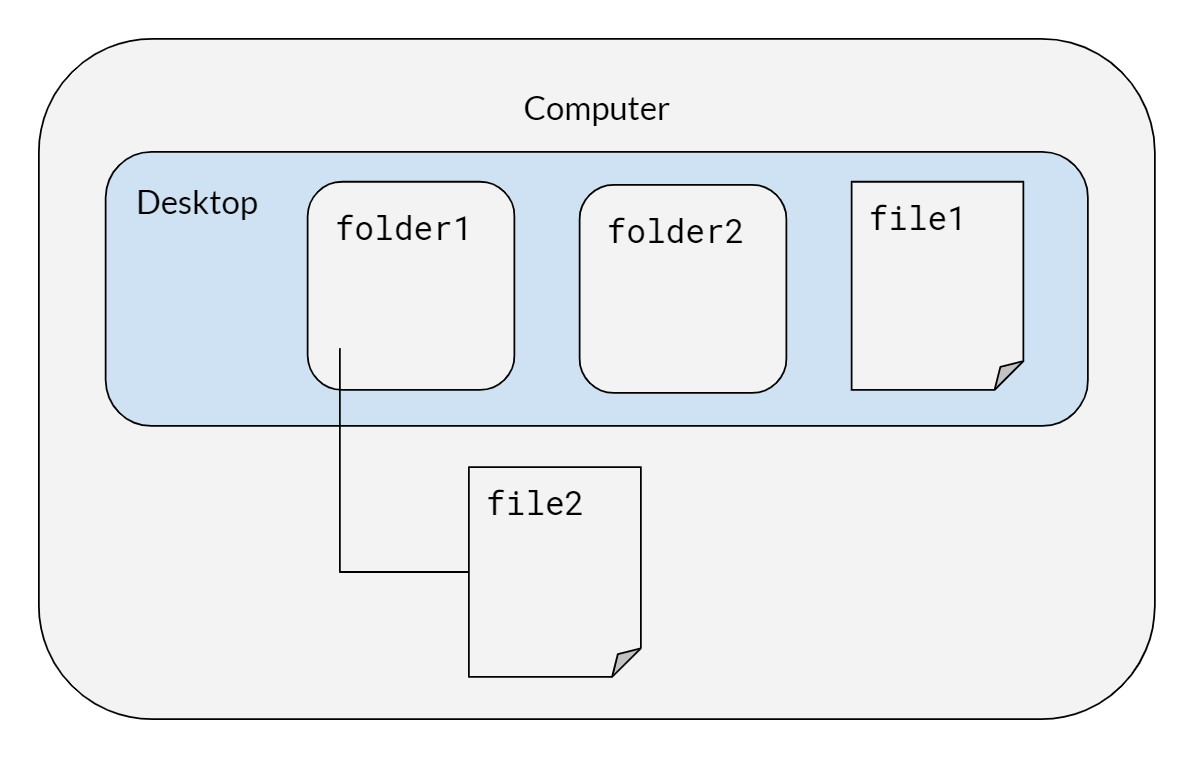
\includegraphics{assets/images/ex-desktop.jpg}
\caption{Here is our example desktop.}
\end{figure}

\section{Syntax for both Mac/Windows}\label{syntax-for-both-macwindows}

When typing in directories or file names, quotes are necessary if the
name includes spaces.

\begin{longtable}[]{@{}ll@{}}
\toprule
\begin{minipage}[b]{0.14\columnwidth}\raggedright\strut
Command\strut
\end{minipage} & \begin{minipage}[b]{0.18\columnwidth}\raggedright\strut
Description\strut
\end{minipage}\tabularnewline
\midrule
\endhead
\begin{minipage}[t]{0.14\columnwidth}\raggedright\strut
\texttt{cd\ desktop/folder1}\strut
\end{minipage} & \begin{minipage}[t]{0.18\columnwidth}\raggedright\strut
Change directory to \texttt{folder1}\strut
\end{minipage}\tabularnewline
\begin{minipage}[t]{0.14\columnwidth}\raggedright\strut
\texttt{pwd}\strut
\end{minipage} & \begin{minipage}[t]{0.18\columnwidth}\raggedright\strut
Print working directory\strut
\end{minipage}\tabularnewline
\begin{minipage}[t]{0.14\columnwidth}\raggedright\strut
\texttt{ls}\strut
\end{minipage} & \begin{minipage}[t]{0.18\columnwidth}\raggedright\strut
List files in the directory\strut
\end{minipage}\tabularnewline
\begin{minipage}[t]{0.14\columnwidth}\raggedright\strut
\texttt{cp\ "file2"\ "newfile2"}\strut
\end{minipage} & \begin{minipage}[t]{0.18\columnwidth}\raggedright\strut
Copy file (remember to include file extensions when typing in file names
like \texttt{.pdf} or \texttt{.R})\strut
\end{minipage}\tabularnewline
\begin{minipage}[t]{0.14\columnwidth}\raggedright\strut
\texttt{mv\ “newfile2”\ “file3”}\strut
\end{minipage} & \begin{minipage}[t]{0.18\columnwidth}\raggedright\strut
Rename \texttt{newfile2} to \texttt{file3}\strut
\end{minipage}\tabularnewline
\begin{minipage}[t]{0.14\columnwidth}\raggedright\strut
\texttt{cd\ ..}\strut
\end{minipage} & \begin{minipage}[t]{0.18\columnwidth}\raggedright\strut
Go to parent of the working directory (in this case,
\texttt{desktop})\strut
\end{minipage}\tabularnewline
\begin{minipage}[t]{0.14\columnwidth}\raggedright\strut
\texttt{mv\ “file1”\ folder2}\strut
\end{minipage} & \begin{minipage}[t]{0.18\columnwidth}\raggedright\strut
Move \texttt{file1} to \texttt{folder2}\strut
\end{minipage}\tabularnewline
\begin{minipage}[t]{0.14\columnwidth}\raggedright\strut
\texttt{mkdir\ folder3}\strut
\end{minipage} & \begin{minipage}[t]{0.18\columnwidth}\raggedright\strut
Make a new folder in \texttt{folder2}\strut
\end{minipage}\tabularnewline
\begin{minipage}[t]{0.14\columnwidth}\raggedright\strut
\texttt{rm\ \textless{}filename\textgreater{}}\strut
\end{minipage} & \begin{minipage}[t]{0.18\columnwidth}\raggedright\strut
Remove files\strut
\end{minipage}\tabularnewline
\begin{minipage}[t]{0.14\columnwidth}\raggedright\strut
\texttt{rm\ -rf\ folder3}\strut
\end{minipage} & \begin{minipage}[t]{0.18\columnwidth}\raggedright\strut
Remove directories (\texttt{-r} will attempt to remove the directory
recursively, \texttt{-rf} will force removal of the directory)\strut
\end{minipage}\tabularnewline
\begin{minipage}[t]{0.14\columnwidth}\raggedright\strut
\texttt{clear}\strut
\end{minipage} & \begin{minipage}[t]{0.18\columnwidth}\raggedright\strut
Clear terminal screen of all previous commands\strut
\end{minipage}\tabularnewline
\bottomrule
\end{longtable}

\begin{figure}
\centering
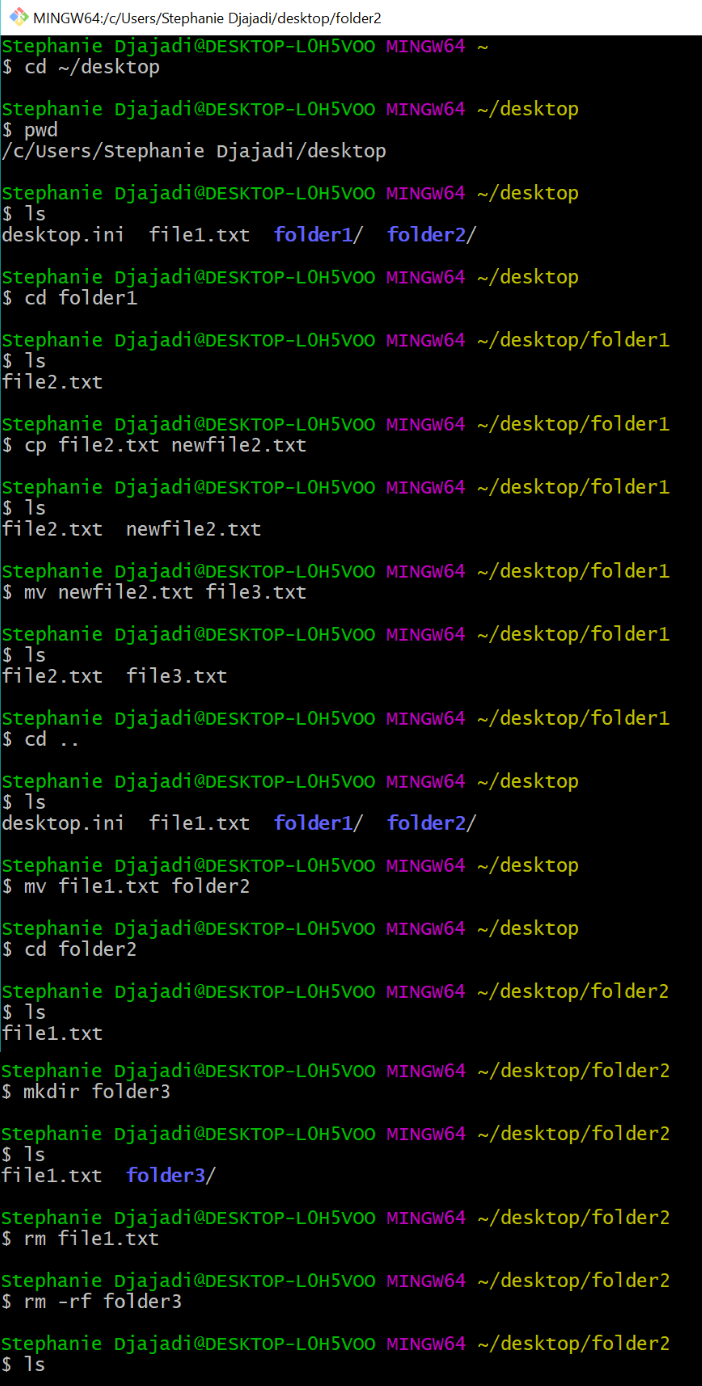
\includegraphics{assets/images/ex-terminal.PNG}
\caption{Here is an example of what your terminal might look like after
executing the commands in the order listed above.}
\end{figure}

\section{Running Bash Scripts}\label{running-bash-scripts}

\begin{longtable}[]{@{}lll@{}}
\toprule
\begin{minipage}[b]{0.13\columnwidth}\raggedright\strut
Windows\strut
\end{minipage} & \begin{minipage}[b]{0.18\columnwidth}\raggedright\strut
Mac / Linux\strut
\end{minipage} & \begin{minipage}[b]{0.18\columnwidth}\raggedright\strut
Description\strut
\end{minipage}\tabularnewline
\midrule
\endhead
\begin{minipage}[t]{0.13\columnwidth}\raggedright\strut
\texttt{chmod\ +750\ \textless{}filename.sh\textgreater{}}\strut
\end{minipage} & \begin{minipage}[t]{0.18\columnwidth}\raggedright\strut
\texttt{chmod\ +x\ \textless{}filename.sh\textgreater{}}\strut
\end{minipage} & \begin{minipage}[t]{0.18\columnwidth}\raggedright\strut
Change access permissions for a file (only needs to be done once)\strut
\end{minipage}\tabularnewline
\begin{minipage}[t]{0.13\columnwidth}\raggedright\strut
\texttt{./\textless{}filename.sh\textgreater{}}\strut
\end{minipage} & \begin{minipage}[t]{0.18\columnwidth}\raggedright\strut
\texttt{./\textless{}filename.sh\textgreater{}}\strut
\end{minipage} & \begin{minipage}[t]{0.18\columnwidth}\raggedright\strut
Run file (\texttt{./} to run any executable file)\strut
\end{minipage}\tabularnewline
\begin{minipage}[t]{0.13\columnwidth}\raggedright\strut
\texttt{bash\ bash\_script\_name.sh\ \&}\strut
\end{minipage} & \begin{minipage}[t]{0.18\columnwidth}\raggedright\strut
\texttt{bash\ bash\_script\_name.sh\ \&}\strut
\end{minipage} & \begin{minipage}[t]{0.18\columnwidth}\raggedright\strut
Run shell script in the background\strut
\end{minipage}\tabularnewline
\bottomrule
\end{longtable}

\section{Running Rscripts in Windows}\label{running-rscripts-in-windows}

\textbf{Note: This code seems to work only with Windows Command Prompt,
not with Git Bash.}

When R is installed, it comes with a utility called Rscript. This allows
you to run R commands from the command line. If Rscript is in your
\texttt{PATH,} then typing Rscript into the command line, and pressing
enter, will not error. Otherwise, to use Rscript, you will either need
to add it to your PATH (as an environment variable), or append the full
directory of the location of Rscript on your machine. To find the full
directory, search for where R is installed your computer. For instance,
it may be something like below (this will vary depending on what version
of R you have installed):

\texttt{C:\textbackslash{}Program\ Files\textbackslash{}R\textbackslash{}R-3.6.0\textbackslash{}bin}

For appending the \texttt{PATH} variable, please view
\href{https://www.howtogeek.com/118594/how-to-edit-your-system-path-for-easy-command-line-access/}{this
link}. I strongly recommend completing this option.

If you add the PATH as an environment variable, then you can run this
line of code to test: \texttt{Rscript\ -e\ “cat(‘this\ is\ a\ test’)"},
where the \texttt{-e} flag refers to the expression that will be
executed.

If you do not add the PATH as an environment variable, then you can run
this line of code to replicate the results from above:
\texttt{“C:\textbackslash{}Program\ Files\textbackslash{}R\textbackslash{}R-3.6.0\textbackslash{}bin”\ -e\ “cat(‘this\ is\ a\ test’)”}

To run an R script from the command line, we can say:
\texttt{Rscript\ -e\ “source(‘C:/path/to/script/some\_code.R’)”}

\subsection{Common Mistakes}\label{common-mistakes}

\begin{itemize}
\tightlist
\item
  Remember to include all of the quotation marks around file paths that
  have a spaces.
\item
  If you attempt to run an R script but run into
  \texttt{Error:\ \textquotesingle{}\textbackslash{}U\textquotesingle{}\ used\ without\ hex\ digits\ in\ character\ string\ starting\ "\textquotesingle{}C:\textbackslash{}U"},
  try replacing all \texttt{\textbackslash{}} with
  \texttt{\textbackslash{}\textbackslash{}} or \texttt{/}.
\end{itemize}

\section{Checking tasks and killing
jobs}\label{checking-tasks-and-killing-jobs}

\begin{longtable}[]{@{}lll@{}}
\toprule
\begin{minipage}[b]{0.13\columnwidth}\raggedright\strut
Windows\strut
\end{minipage} & \begin{minipage}[b]{0.18\columnwidth}\raggedright\strut
Mac / Linux\strut
\end{minipage} & \begin{minipage}[b]{0.18\columnwidth}\raggedright\strut
Description\strut
\end{minipage}\tabularnewline
\midrule
\endhead
\begin{minipage}[t]{0.13\columnwidth}\raggedright\strut
\texttt{tasklist}\strut
\end{minipage} & \begin{minipage}[t]{0.18\columnwidth}\raggedright\strut
\texttt{ps\ -v}\strut
\end{minipage} & \begin{minipage}[t]{0.18\columnwidth}\raggedright\strut
List all processes on the command line\strut
\end{minipage}\tabularnewline
\begin{minipage}[t]{0.13\columnwidth}\raggedright\strut
\strut
\end{minipage} & \begin{minipage}[t]{0.18\columnwidth}\raggedright\strut
\texttt{top\ -o\ {[}cpu/rsize{]}}\strut
\end{minipage} & \begin{minipage}[t]{0.18\columnwidth}\raggedright\strut
List all running processes, sorted by CPU or memory usage\strut
\end{minipage}\tabularnewline
\begin{minipage}[t]{0.13\columnwidth}\raggedright\strut
\texttt{taskkill\ /F\ /PID\ pid\_number}\strut
\end{minipage} & \begin{minipage}[t]{0.18\columnwidth}\raggedright\strut
\texttt{kill\ \textless{}PID\_number\textgreater{}}\strut
\end{minipage} & \begin{minipage}[t]{0.18\columnwidth}\raggedright\strut
Kill a process by its process ID\strut
\end{minipage}\tabularnewline
\begin{minipage}[t]{0.13\columnwidth}\raggedright\strut
\texttt{taskkill\ /IM\ "process\ name"\ /F}\strut
\end{minipage} & \begin{minipage}[t]{0.18\columnwidth}\raggedright\strut
\strut
\end{minipage} & \begin{minipage}[t]{0.18\columnwidth}\raggedright\strut
Kill a process by its name\strut
\end{minipage}\tabularnewline
\begin{minipage}[t]{0.13\columnwidth}\raggedright\strut
\texttt{start\ /b\ program.exe}\strut
\end{minipage} & \begin{minipage}[t]{0.18\columnwidth}\raggedright\strut
\strut
\end{minipage} & \begin{minipage}[t]{0.18\columnwidth}\raggedright\strut
Runs jobs in the background (exclude \texttt{/b} if you want the program
to run in a new console)\strut
\end{minipage}\tabularnewline
\begin{minipage}[t]{0.13\columnwidth}\raggedright\strut
\strut
\end{minipage} & \begin{minipage}[t]{0.18\columnwidth}\raggedright\strut
\texttt{nohup}\strut
\end{minipage} & \begin{minipage}[t]{0.18\columnwidth}\raggedright\strut
Prevents jobs from stopping\strut
\end{minipage}\tabularnewline
\begin{minipage}[t]{0.13\columnwidth}\raggedright\strut
\strut
\end{minipage} & \begin{minipage}[t]{0.18\columnwidth}\raggedright\strut
\texttt{disown}\strut
\end{minipage} & \begin{minipage}[t]{0.18\columnwidth}\raggedright\strut
Keeps jobs running in the background even if you close R\strut
\end{minipage}\tabularnewline
\begin{minipage}[t]{0.13\columnwidth}\raggedright\strut
\texttt{taskkill\ /?}\strut
\end{minipage} & \begin{minipage}[t]{0.18\columnwidth}\raggedright\strut
\strut
\end{minipage} & \begin{minipage}[t]{0.18\columnwidth}\raggedright\strut
Help, lists out other commands\strut
\end{minipage}\tabularnewline
\bottomrule
\end{longtable}

To kill a task in Windows, you can also go to Task Manager
\textgreater{} More details \textgreater{} Select your desired app
\textgreater{} Click on End Task.

\section{Running big jobs}\label{running-big-jobs}

For big data workflows, the concept of ``backgrounding'' a bash script
allows you to start a ``job'' (i.e.~run the script) and leave it
overnight to run. At the top level, a bash script
(\texttt{0-run-project.sh}) that simply calls the directory-level bash
scripts (i.e. \texttt{0-prep-data.sh}, \texttt{0-run-analysis.sh},
\texttt{0-run-figures.sh}, etc.) is a powerful tool to rerun every
script in your project. See the included example bash scripts for more
details.

\begin{itemize}
\tightlist
\item
  \textbf{Running Bash Scripts in Background}: Running a long bash
  script is not trivial. Normally you would run a bash script by opening
  a terminal and typing something like \texttt{./run-project.sh}. But
  what if you leave your computer, log out of your server, or close the
  terminal? Normally, the bash script will exit and fail to complete. To
  run it in background, type \texttt{./run-project.sh\ \&;\ disown}. You
  can see the job running (and CPU utilization) with the command
  \texttt{top} or \texttt{ps\ -v} and check your memory with
  \texttt{free\ -h}.
\end{itemize}

Alternatively, to keep code running in the background even when an SSH
connection is broken, you can use \texttt{tmux}. In terminal or gitbash
follow the steps below. This
\href{https://medium.com/@jeongwhanchoi/install-tmux-on-osx-and-basics-commands-for-beginners-be22520fd95e}{site}
has useful tips on using \texttt{tmux}.

\begin{verbatim}
# create a new tmux session called session_name
tmux new -ssession_name

# run your job of interest
R CMD BATCH myjob.R & 
  
# check that it is running
ps -v

# to exit the tmux session (Mac)
ctrl + b 
d

# to reopen the tmux session to kill the job or 
# start another job
tmux attach -tsession_name 
\end{verbatim}

\begin{itemize}
\item
  \textbf{Deleting Previously Computed Results}: One helpful lesson
  we've learned is that your bash scripts should remove previous results
  (computed and saved by scripts run at a previous time) so that you
  never mix results from one run with a previous run. This can happen
  when an R script errors out before saving its result, and can be
  difficult to catch because your previously saved result exists
  (leading you to believe everything ran correctly).
\item
  \textbf{Ensuring Things Ran Correctly}: You should check the
  \texttt{.Rout} files generated by the R scripts run by your bash
  scripts for errors once things are run. A utility file is include in
  this repository, called \texttt{runFileSaveLogs}, and is used by the
  example bash scripts to\ldots{} run files and save the generated logs.
  It is an awesome utility and one I definitely recommend using. Before
  using \texttt{runFileSaveLogs}, it is necessary to put the file in the
  home working directory. For help and documentation, you can use the
  command \texttt{./runFileSaveLogs\ -h}. See example code and example
  usage for \texttt{runFileSaveLogs} below.
\end{itemize}

\subsection{\texorpdfstring{Example code for
\texttt{runfileSaveLogs}}{Example code for runfileSaveLogs}}\label{example-code-for-runfilesavelogs}

\begin{Shaded}
\begin{Highlighting}[]
\CommentTok{#!/usr/bin/env python3}
\CommentTok{# Type "./runFileSaveLogs -h" for help}

\ImportTok{import}\NormalTok{ os}
\ImportTok{import}\NormalTok{ sys}
\ImportTok{import}\NormalTok{ argparse}
\ImportTok{import}\NormalTok{ getpass}
\ImportTok{import}\NormalTok{ datetime}
\ImportTok{import}\NormalTok{ shutil}
\ImportTok{import}\NormalTok{ glob}
\ImportTok{import}\NormalTok{ pathlib}

\CommentTok{# Setting working directory to this script's current directory}
\NormalTok{os.chdir(os.path.dirname(os.path.abspath(}\VariableTok{__file__}\NormalTok{)))}

\CommentTok{# Setting up argument parser}
\NormalTok{parser }\OperatorTok{=}\NormalTok{ argparse.ArgumentParser(description}\OperatorTok{=}\StringTok{'Runs the argument R script(s) - in parallel if specified - and moves the subsequent generated .Rout log files to a timestamped directory.'}\NormalTok{)}

\CommentTok{# Function ensuring that the file is valid}
\KeywordTok{def}\NormalTok{ is_valid_file(parser, arg):}
    \ControlFlowTok{if} \KeywordTok{not}\NormalTok{ os.path.exists(arg):}
\NormalTok{        parser.error(}\StringTok{"The file }\SpecialCharTok\NormalTok{ arg)}
    \ControlFlowTok{else}\NormalTok{:}
        \ControlFlowTok{return}\NormalTok{ arg}

\CommentTok{# Function ensuring that the directory is valid}
\KeywordTok{def}\NormalTok{ is_valid_directory(parser, arg):}
    \ControlFlowTok{if} \KeywordTok{not}\NormalTok{ os.path.isdir(arg):}
\NormalTok{        parser.error(}\StringTok{"The specified path (}\SpecialCharTok\NormalTok{ arg)}
    \ControlFlowTok{else}\NormalTok{:}
        \ControlFlowTok{return}\NormalTok{ arg}

\CommentTok{# Additional arguments that can be added when running runFileSaveLogs}
\NormalTok{parser.add_argument(}\StringTok{'-p'}\NormalTok{, }\StringTok{'--parallel'}\NormalTok{, action}\OperatorTok{=}\StringTok{'store_true'}\NormalTok{, }\BuiltInTok{help}\OperatorTok{=}\StringTok{"Runs the argument R scripts in parallel if specified"}\NormalTok{)}
\NormalTok{parser.add_argument(}\StringTok{"-i"}\NormalTok{, }\StringTok{"--identifier"}\NormalTok{, }\BuiltInTok{help}\OperatorTok{=}\StringTok{"Adds an identifier to the directory name where this is saved"}\NormalTok{)}
\NormalTok{parser.add_argument(}\StringTok{'filenames'}\NormalTok{, nargs}\OperatorTok{=}\StringTok{'+'}\NormalTok{, }\BuiltInTok{type}\OperatorTok{=}\KeywordTok{lambda}\NormalTok{ x: is_valid_file(parser, x))}

\NormalTok{args }\OperatorTok{=}\NormalTok{ parser.parse_args()}
\NormalTok{args_dict }\OperatorTok{=} \BuiltInTok{vars}\NormalTok{(args)}

\BuiltInTok{print}\NormalTok{(args_dict)}

\CommentTok{# Run given R Scripts}
\ControlFlowTok{for}\NormalTok{ filename }\KeywordTok{in}\NormalTok{ args_dict[}\StringTok{"filenames"}\NormalTok{]:}
\NormalTok{  system_call }\OperatorTok{=} \StringTok{"R CMD BATCH"} \OperatorTok{+} \StringTok{" "} \OperatorTok{+}\NormalTok{ filename}
  \ControlFlowTok{if}\NormalTok{ args_dict[}\StringTok{"parallel"}\NormalTok{]: }
\NormalTok{    system_call }\OperatorTok{=} \StringTok{"nohup"} \OperatorTok{+} \StringTok{" "} \OperatorTok{+}\NormalTok{ system_call }\OperatorTok{+} \StringTok{" &"}

\NormalTok{  os.system(system_call)}

\CommentTok{# Create the directory (and any parents) of the log files}
\NormalTok{currentUser }\OperatorTok{=}\NormalTok{ getpass.getuser()}
\NormalTok{currentTime }\OperatorTok{=}\NormalTok{ datetime.datetime.now().strftime(}\StringTok{"%Y-%m-}\SpecialCharTok{%d}\StringTok{ %H:%M:%S"}\NormalTok{)}
\NormalTok{logDirPrefix }\OperatorTok{=} \StringTok{"/home/kaiserData/logs/"} \CommentTok{# Change to the directory where the logs should be saved}
\NormalTok{logDir }\OperatorTok{=}\NormalTok{ logDirPrefix }\OperatorTok{+}\NormalTok{ currentTime }\OperatorTok{+} \StringTok{"-"} \OperatorTok{+}\NormalTok{ currentUser }

\CommentTok{# If specified, adds the identifier to the filename of the log}
\ControlFlowTok{if}\NormalTok{ args.identifier }\KeywordTok{is} \KeywordTok{not} \VariableTok{None}\NormalTok{:}
\NormalTok{  logDir }\OperatorTok{+=} \StringTok{"-"} \OperatorTok{+}\NormalTok{ args.identifier}

\NormalTok{logDir }\OperatorTok{+=} \StringTok{"/"}

\NormalTok{pathlib.Path(logDir).mkdir(parents}\OperatorTok{=}\VariableTok{True}\NormalTok{, exist_ok}\OperatorTok{=}\VariableTok{True}\NormalTok{)}

\CommentTok{# Find and move all logs to this new directory}
\NormalTok{currentLogPaths }\OperatorTok{=}\NormalTok{ glob.glob(}\StringTok{'./*.Rout'}\NormalTok{)}

\ControlFlowTok{for}\NormalTok{ currentLogPath }\KeywordTok{in}\NormalTok{ currentLogPaths:}
\NormalTok{  filename }\OperatorTok{=}\NormalTok{ currentLogPath.split(}\StringTok{"/"}\NormalTok{)[}\OperatorTok{-}\DecValTok{1}\NormalTok{]}
\NormalTok{  shutil.move(currentLogPath, logDir }\OperatorTok{+}\NormalTok{ filename)}
\end{Highlighting}
\end{Shaded}

\subsection{\texorpdfstring{Example usage for
\texttt{runfileSaveLogs}}{Example usage for runfileSaveLogs}}\label{example-usage-for-runfilesavelogs}

This example bash script runs files and generates logs for five scripts
in the \texttt{kaiserflu/3-figures} folder. Note that the \texttt{-i}
flag is used as an identifier to add \texttt{figures} to the filename of
each log.

\begin{verbatim}
#!/bin/bash

# Copy utility run script into this folder for concision in call
cp ~/kaiserflu/runFileSaveLogs ~/kaiserflu/3-figures/

# Run folder scripts and produce output
cd ~/kaiserflu/3-figures/
./runFileSaveLogs -i "figures" \
fig-mean-season-age.R \
fig-monthly-rate.R \
fig-point-estimates-combined.R \
fig-point-estimates.R \
fig-weekly-rate.R

# Remove copied utility run script
rm runFileSaveLogs
\end{verbatim}

\chapter{Resources}\label{resources}

by Jade Benjamin-Chung and Kunal Mishra

\section{Resources for R}\label{resources-for-r}

\begin{itemize}
\tightlist
\item
  \href{https://www.rstudio.com/wp-content/uploads/2015/02/data-wrangling-cheatsheet.pdf}{dplyr
  and tidyr cheat sheet}
\item
  \href{https://www.rstudio.com/wp-content/uploads/2015/03/ggplot2-cheatsheet.pdf}{ggplot
  cheat sheet}
\item
  \href{https://s3.amazonaws.com/assets.datacamp.com/blog_assets/datatable_Cheat_Sheet_R.pdf}{data
  table cheat sheet}
\item
  \href{https://www.rstudio.com/wp-content/uploads/2015/02/rmarkdown-cheatsheet.pdf}{RMarkdown
  cheat sheet}
\item
  \href{http://adv-r.had.co.nz/Style.html}{Hadley Wickham's R Style
  Guide}
\item
  \href{https://ucb-epi-r.github.io}{Jade's R-for-epi course}
\item
  \href{https://www.youtube.com/watch?v=nERXS3ssntw}{Tidy Eval in 5
  Minutes} (video)
\item
  \href{https://tidyeval.tidyverse.org/index.html}{Tidy Evaluation}
  (e-book)
\item
  \href{https://www.brodrigues.co/blog/2016-07-18-data-frame-columns-as-arguments-to-dplyr-functions/}{Data
  Frame Columns as Arguments to Dplyr Functions} (blog)
\item
  \href{https://stackoverflow.com/questions/28125816/r-standard-evaluation-for-join-dplyr}{Standard
  Evaluation for *\_join} (stackoverflow)
\item
  \href{https://dplyr.tidyverse.org/articles/programming.html}{Programming
  with dplyr} (package vignette)
\end{itemize}

\section{Resources for Github}\label{resources-for-github}

\section{Authorship}\label{authorship}

\begin{itemize}
\tightlist
\item
  \href{http://www.icmje.org/recommendations/browse/roles-and-responsibilities/defining-the-role-of-authors-and-contributors.html}{ICMJE
  Definition of authorship}
\end{itemize}

\bibliography{book.bib,packages.bib}

\end{document}
